\documentclass[journal,10pt,twocolumn]{IEEEtran}

% Essential Packages
\usepackage[utf8]{inputenc}
\usepackage[T1]{fontenc}
\usepackage{amsmath,amssymb,amsfonts}
\usepackage{booktabs}
\usepackage{graphicx}
\usepackage{float}
\usepackage{cite}
\usepackage{xcolor}
\usepackage[hyphens]{url}
\usepackage[protrusion=true,expansion=false]{microtype}
\usepackage[hidelinks]{hyperref}

% Compatibility macros for citations
\providecommand{\citep}[1]{\cite{#1}}
\providecommand{\citet}[1]{\cite{#1}}

% Graphics path
\graphicspath{{../results/figures/}{results/figures/}}

\title{Predictive Maintenance and Anomaly Detection for Industrial IoT Telemetry Using Machine Learning: A Rigorous Empirical Study on NASA C-MAPSS under Leakage-Free Protocols}

\author{Rahul~Xiao%
\thanks{Manuscript received October 8, 2026. This research was conducted under the project ``Predictive Maintenance and Anomaly Detection for Industrial IoT Telemetry Using Machine Learning''.}%
\thanks{The author is with the Department of Computer Science and Engineering (e-mail: rahul.xiao@example.org). Code, datasets, and verification manifests are available at \url{https://github.com/rahulxiao/Predictive-Maintenance-IoT-Telemetry}.}%
}

\begin{document}

\maketitle

\begin{abstract}
Predictive maintenance (PdM) of critical cyber-physical systems relies on detecting incipient degradation and forecasting Remaining Useful Life (RUL) from multi-sensor telemetry. On the canonical NASA Commercial Modular Aero-Propulsion System Simulation (C-MAPSS) turbofan benchmark (FD001--FD004), modern machine learning (ML) architectures consistently achieve high diagnostic accuracy. However, standard evaluation protocols suffer from critical methodological vulnerabilities, including evaluation-fold tuning optimism, cross-condition normalization leakage, and circular lead-time definitions where warnings trivially track supervised classification cutoffs ($RUL \le N$).

This paper presents a rigorous empirical investigation into anomaly detection and prognostic forecasting under strictly leakage-free conditions. Using 5-fold shuffled \texttt{GroupKFold} unit splits over 5 random seeds, we benchmark Random Forests, XGBoost, Deep 1D-CNNs, and LSTMs against condition-aware statistical baselines ($k$-sigma static thresholds and EWMA control limits) and unsupervised health indices. On official test engines, supervised ML achieves dominant window-level classification ($F_1 = 0.753$--$0.858$, PR-AUC $= 0.826$--$0.938$) and accurate RUL prediction (LSTM RMSE $13.98 \pm 0.22$ on FD003; XGBoost RMSE $29.60 \pm 0.15$ on FD004). 

Crucially, operating characteristic sweeps demonstrate that the tuned static threshold warns earlier than ML detectors under zero or minimal false alarms on multi-fault/multi-regime subsets (median difference $-3.0$ cycles on FD003, Holm-corrected $p = 0.0264$). Furthermore, sensitivity sweeps over $N \in \{20, 30, 50, 75, 100\}$ prove that supervised lead times are strictly circular, tracking $N$ rather than physical degradation onset. Split conformal prediction intervals achieve $73.7\%$--$84.0\%$ empirical test coverage at $90\%$ target coverage, and TreeSHAP confirms $60\%$--$80\%$ feature attribution consensus with physical control charts.
\end{abstract}

\begin{IEEEkeywords}
Predictive maintenance, remaining useful life (RUL), anomaly detection, industrial IoT, turbofan telemetry, NASA C-MAPSS, conformal prediction, domain adaptation, TreeSHAP.
\end{IEEEkeywords}


\section{Introduction}
\label{sec:introduction}

\subsection{Motivation}
In modern industrial cyber-physical infrastructure---ranging from civil aviation propulsion systems to renewable power generation fleets---unexpected component failures incur catastrophic economic losses, unplanned operational downtime, and severe safety hazards. The proliferation of Industrial Internet of Things (IIoT) architectures has facilitated continuous, high-frequency telemetry acquisition across fleets of rotating machinery. Consequently, Predictive Maintenance (PdM) and Prognostics and Health Management (PHM) have shifted from retrospective breakdown repairs and calendar-based preventative servicing toward continuous condition-based prognostics \cite{saxena2008damage, ramasso2014performance}.

The core operational objective of predictive maintenance is twofold:
\begin{enumerate}
    \item \textbf{Early Anomaly Warning}: Detecting the earliest physical transition from nominal, healthy operation to an anomalous, degrading state, providing maintenance operators with sufficient warning lead time while constraining false alarm rates.
    \item \textbf{Prognostic Horizon Forecasting}: Accurately estimating the Remaining Useful Life (RUL) of the asset, defined as the number of operational cycles or operating hours remaining before component failure.
\end{enumerate}

The canonical benchmark for evaluating data-driven PdM methodologies is the NASA Commercial Modular Aero-Propulsion System Simulation (C-MAPSS) dataset suite \cite{saxena2008damage}. C-MAPSS provides high-dimensional run-to-failure telemetry across four subsets (FD001 through FD004), encompassing single and multi-regime operating conditions as well as single and dual fault modes.

\subsection{Problem Statement and Evaluation Vulnerabilities}
Despite a decade of literature applying deep neural networks, ensemble tree methods, and recurrent architectures to C-MAPSS, published evaluations suffer from pervasive methodological vulnerabilities that threaten real-world validity:
\begin{enumerate}
    \item \textbf{Circular Warning Lead Times}: In supervised classification studies, anomaly labels are commonly assigned by designating cycles where $RUL \le N$ (typically $N=30$) as ``anomalous''. When an evaluation claims an early warning lead time of 28 cycles before failure, this metric is fundamentally circular: it reflects the arbitrary choice of $N=30$ rather than the physical onset of degradation.
    \item \textbf{Optimistic Baseline Evaluation}: Many comparative studies benchmark complex deep architectures against uncalibrated or improperly tuned statistical baselines, failing to condition control charts on operating regimes or evaluating baselines under mismatched false alarm rates.
    \item \textbf{Cross-Condition Telemetry Leakage}: In multi-condition datasets (FD002, FD004), operating regimes dramatically distort sensor telemetry. In literature, normalization statistics are frequently fit across the entire dataset or fit on the target domain during cross-condition transfer, masking catastrophic domain shift.
    \item \textbf{Lack of Rigorous Statistical Correction}: Multiple comparative hypothesis tests are frequently published without Family-Wise Error Rate (FWER) corrections, leading to spurious claims of algorithmic superiority.
\end{enumerate}

\subsection{Research Questions}
To address these fundamental challenges, this paper investigates four central research questions:
\begin{description}
    \item[\textbf{RQ1}] \textbf{Prognostic and Diagnostic Accuracy}: How accurately can machine learning architectures identify anomalies and forecast degradation (RUL) across single-condition and multi-condition industrial telemetry fleets?
    \item[\textbf{RQ2}] \textbf{Machine Learning vs. Statistical Baselines}: How do machine learning models perform relative to condition-aware moving-average (EWMA) and static-threshold ($k$-sigma) baselines when evaluated at strictly equal false alarm rates across full trajectories?
    \item[\textbf{RQ3}] \textbf{Achievable Early Warning Lead Time}: What maximum warning lead time is reliably achievable in industrial telemetry fleets, at what false alarm rate, and how does supervised label definition ($N$) constrain achievable lead times?
    \item[\textbf{RQ4}] \textbf{Optimal Preprocessing and Dimensionality Reduction}: Which signal preprocessing techniques (temporal smoothing) and feature representations (raw flattened windows vs. PCA dimensionality reduction vs. summary statistics engineering) yield superior prognostic and diagnostic performance?
\end{description}

\subsection{Contributions}
The key contributions of this work are as follows:
\begin{itemize}
    \item \textbf{Leakage-Free Standardized Benchmark Pipeline}: A fully reproducible evaluation architecture implementing 5-fold shuffled \texttt{GroupKFold} by engine unit across 5 random seeds (0--4), guaranteeing zero test engine data leakage and seed-varying fold splits.
    \item \textbf{Unconstrained Lead-Time Operating Curves}: Sweep-based evaluation of warning lead time vs. false alarms per 100 healthy cycles across 7 methods (Static Threshold, EWMA, Mahalanobis Health Index, Isolation Forest, Random Forest, XGBoost, and LSTM), establishing reliable lead times at controlled industrial false alarm budgets ($\text{FA} \in \{0.1, 0.5, 1.0\}$).
    \item \textbf{Empirical Proof of Supervised Circularity}: A systematic label sensitivity sweep across $N \in \{20, 30, 50, 75, 100\}$ demonstrating that supervised alarm lead time tracks $N$ rather than physical damage, while proving that expanding $N \ge 75$ causes false alarm rates to escalate to $25.7$ per 100 cycles.
    \item \textbf{Identification of the Baseline Warning Lead-Time Paradox}: Discovery that while ML models vastly outperform statistical baselines in window-level classification ($F_1 = 0.753$--$0.858$ vs. $0.336$--$0.671$), a tuned regime-normalized static threshold warns earlier than ML models on multi-fault/multi-regime fleets under minimal false alarms ($p = 0.0264$ on FD003).
    \item \textbf{Cross-Condition Generalization Quantification}: Rigorous evaluation of cross-condition transfer (FD001 $\to$ FD002/FD004, FD003 $\to$ FD004) with normalizers fit strictly on the training domain, revealing a $103\%$ increase in RUL RMSE and a collapse of $F_1$ from $0.797$ down to $0.099$.
    \item \textbf{Distribution-Free Uncertainty Quantification}: Implementation of split conformal prediction intervals calibrated on whole held-out train engines at $90\%$ target coverage, reporting empirical test coverage and interval widths.
    \item \textbf{Physical Explainability}: TreeSHAP feature attributions on XGBoost demonstrating $60\%$--$80\%$ consensus with the sensors driving statistical control charts, identifying High-Pressure Compressor (HPC) outlet static pressure (\texttt{s11}) as the primary wear indicator.
\end{itemize}

\subsection{Paper Organization}
The remainder of this paper is organized as follows: Section~\ref{sec:related_work} reviews related literature in prognostic modeling and baseline benchmarking. Section~\ref{sec:dataset} presents the NASA C-MAPSS dataset suite and condition-aware regime normalization. Section~\ref{sec:methodology} formalizes the predictive architectures, evaluation protocols, and conformal calibration. Section~\ref{sec:experiments} presents comprehensive empirical findings across all experimental phases. Section~\ref{sec:discussion} analyzes the baseline paradox, lead-time circularity, and operational implications. Section~\ref{sec:limitations} evaluates methodological limitations, and Section~\ref{sec:conclusion} concludes.

\section{Related Work}
\label{sec:related_work}

\subsection{Predictive Maintenance and the C-MAPSS Benchmark}
Predictive maintenance has evolved from statistical reliability analysis toward data-driven prognostic modeling leveraging deep learning and ensemble trees \cite{saxena2008damage}. The NASA Commercial Modular Aero-Propulsion System Simulation (C-MAPSS) turbofan benchmark was introduced by Saxena et al. \cite{saxena2008damage} to simulate realistic damage propagation in gas turbine engines. C-MAPSS couples aerothermal physics with stochastic degradation modeling, capturing component wear across fan, low-pressure compressor (LPC), high-pressure compressor (HPC), high-pressure turbine (HPT), and low-pressure turbine (LPT) assemblies.

In the inaugural 2008 IEEE PHM Data Challenge using C-MAPSS, Heimes \cite{heimes2008recurrent} demonstrated the efficacy of recurrent neural networks (RNNs) for RUL regression, winning the competitive challenge by training backpropagation networks directly on flight trajectories. Later, Ramasso and Saxena \cite{ramasso2014performance} conducted an exhaustive benchmarking analysis across prognostic methodologies on C-MAPSS, establishing standardized piecewise linear degradation assumptions (capping nominal RUL at an upper threshold, typically 125 cycles) and identifying the pronounced performance discrepancies between single-regime datasets (FD001, FD003) and multi-regime datasets (FD002, FD004).

\subsection{Deep Learning for Remaining Useful Life Estimation}
With the resurgence of deep representation learning, time-series neural networks have become dominant in C-MAPSS literature:
\begin{itemize}
    \item \textbf{Recurrent Architectures}: Zheng et al. \cite{zheng2017long} introduced Long Short-Term Memory (LSTM) networks for C-MAPSS RUL regression. By propagating hidden states across sliding windows, LSTMs naturally capture long-term temporal dependencies in sensor degradation trajectories without requiring manual feature engineering.
    \item \textbf{Convolutional Architectures}: Babu et al. \cite{babu2016deep} established the application of deep 2D/1D Convolutional Neural Networks (CNNs) for prognostic regression on C-MAPSS, applying temporal filter kernels across sensor dimensions. Li et al. \cite{li2018remaining} extended this approach using deep 1D-CNNs with time-windowing, demonstrating that convolutional feature maps extract localized sensor degradation patterns while maintaining computational throughput superior to recurrent networks.
\end{itemize}

\subsection{Tree Ensembles and Industrial Practice}
In real-world IIoT deployments, gradient-boosted decision trees, particularly XGBoost \cite{chen2016xgboost}, remain widely utilized due to their computational efficiency, robustness against hyperparameter sensitivity, and natural handling of tabular statistical features. When paired with windowed summary feature extraction (e.g., temporal means, standard deviations, and trend slopes), tree ensembles achieve prognostic accuracy rivaling deep neural networks while executing in a fraction of the training time \cite{chen2016xgboost}.

\subsection{Statistical Process Control and Baselines}
Despite widespread adoption of deep neural networks, classical Statistical Process Control (SPC) charts remain the foundational standard in industrial operational monitoring \cite{montgomery2009introduction}. Shewhart static $k$-sigma control charts and Exponentially Weighted Moving Average (EWMA) control limits filter sensor telemetry to detect shifts in mean operating levels. While conventional C-MAPSS papers frequently omit statistical baselines or benchmark against un-tuned, un-normalized threshold detectors, condition-aware baselines paired with persistence filtering (requiring consecutive out-of-control cycles) provide strong benchmarks for anomaly warning \cite{montgomery2009introduction}.

\subsection{Uncertainty Quantification and Conformal Prediction}
A fundamental limitation of deterministic RUL regression models is the absence of rigorous uncertainty quantification. In safety-critical aerospace operations, a point estimate $\hat{y}$ is insufficient for decision-making without reliable confidence bounds. Conformal prediction, formalized by Angelopoulos and Bates \cite{angelopoulos2021gentle}, provides distribution-free, finite-sample prediction intervals with mathematically guaranteed marginal coverage. By calibrating non-conformity scores on held-out calibration units, split conformal prediction generates prediction intervals $[\hat{y} - q, \hat{y} + q]$ without requiring distributional assumptions or Bayesian approximations.

\subsection{Explainability and Multiple Hypothesis Testing}
To transition black-box machine learning models into operational aerospace certification, feature attribution methods such as SHAP (SHapley Additive exPlanations) \cite{lundberg2017unified} have gained widespread adoption. Rooted in cooperative game theory, TreeSHAP computes exact Shapley values for tree ensembles, quantifying each sensor's contribution to degradation estimates.

Finally, when evaluating diagnostic models across multiple subsets and metrics, conducting multiple statistical comparisons inflates Type I error. To preserve statistical integrity, Holm \cite{holm1979simple} established the sequentially rejective step-down Bonferroni-Holm procedure, which controls the Family-Wise Error Rate (FWER) across $M$ hypothesis tests without the extreme conservatism of standard Bonferroni adjustments.

\section{C-MAPSS Dataset and Benchmark Formulation}
\label{sec:dataset}

\subsection{C-MAPSS Turbofan Simulation Architecture}
The NASA C-MAPSS (Commercial Modular Aero-Propulsion System Simulation) benchmark simulates the operation and degradation of a large commercial turbofan engine (nominally in the 90,000-lb thrust class) \cite{saxena2008damage}. Each record in the dataset corresponds to a discrete operational flight cycle and includes:
\begin{itemize}
    \item \textbf{Unit Identifier}: Integer index identifying the individual engine unit in the fleet.
    \item \textbf{Time in Cycles}: Elapsed operational flight cycles from beginning of life until failure (in train sets) or until maintenance truncation (in test sets).
    \item \textbf{Operational Settings}: Three operational flight parameters:
    \begin{itemize}
        \item \texttt{op1}: Flight altitude (0 to 42,000 ft).
        \item \texttt{op2}: Mach number (0.0 to 0.84).
        \item \texttt{op3}: Throttle resolver angle / Power Lever Angle (TRA, 20 to 100).
    \end{itemize}
    \item \textbf{Sensor Telemetry}: 21 sensor measurements capturing physical gas path variables including temperatures (LPC, HPC, LPT, exhaust), pressures (total and static pressures across compressor and turbine stages), rotational speeds (core and fan physical and corrected speeds), and flow ratios.
\end{itemize}

\subsection{Benchmark Subsets Overview}
The C-MAPSS suite comprises four distinct subsets reflecting varying degrees of operational complexity, summarized in Table~\ref{tab:cmapss_subsets}.

\begin{table}[htbp]
\centering
\caption{Characteristics of NASA C-MAPSS Dataset Subsets}
\label{tab:cmapss_subsets}
\begin{tabular}{lcccc}
\toprule
\textbf{Dataset} & \textbf{Op. Cond.} & \textbf{Fault Modes} & \textbf{Train Units} & \textbf{Test Units} \\
\midrule
\textbf{FD001} & 1 (Sea Level) & 1 (HPC Wear) & 100 & 100 \\
\textbf{FD002} & 6 (Envelope) & 1 (HPC Wear) & 260 & 259 \\
\textbf{FD003} & 1 (Sea Level) & 2 (HPC + Fan) & 100 & 100 \\
\textbf{FD004} & 6 (Envelope) & 2 (HPC + Fan) & 249 & 248 \\
\bottomrule
\end{tabular}
\end{table}

\subsection{Sensor Selection and Variance Filtering}
In single-regime datasets (FD001, FD003), several sensors exhibit near-zero variance across the entire engine lifetime due to constant ambient operating conditions. To prevent numerical instability and eliminate uninformative features, sensor selection is conducted strictly on training engines using a variance threshold $\sigma^2 > 0.001$:
\begin{itemize}
    \item In \textbf{FD001} and \textbf{FD003}, 7 sensors exhibit negligible variance (\texttt{s1, s5, s6, s10, s16, s18, s19}), yielding a 14-sensor feature space:
    \begin{align*}
    \mathcal{S}_{\text{common}} = \{&\texttt{s2, s3, s4, s7, s8, s9, s11}, \\
    &\texttt{s12, s13, s14, s15, s17, s20, s21}\}.
    \end{align*}
    \item In \textbf{FD002} and \textbf{FD004}, operating condition fluctuations activate all sensors except sensor \texttt{s16}, yielding 20 informative sensor features.
    \item For cross-condition transfer benchmarking, models are projected onto the 14 sensors shared across all subsets.
\end{itemize}

\subsection{Condition-Aware Operating Regime Normalization}
In multi-condition datasets (FD002, FD004), raw sensor telemetry is dominated by operating setting variations rather than degradation. For example, high-pressure turbine temperature variations due to altitude changes exceed the temperature increases induced by component wear.

To isolate degradation dynamics, we implement condition-aware regime normalization via the \texttt{OperatingRegimeNormalizer}:
\begin{enumerate}
    \item \textbf{Regime Clustering}: For multi-condition sets, the 3 operational settings (\texttt{op1, op2, op3}) are clustered into $K=6$ operating regimes using $k$-means clustering, fit strictly on training engines.
    \item \textbf{Healthy Baseline Calibration}: In physical turbomachinery, initial operational cycles represent nominal healthy health states. The healthy operational phase is defined as the first $30\%$ of life of training engines:
    $$\mathcal{T}_{\text{healthy}} = \{t \in [1, T_{\text{fail}}] : t \le \lfloor 0.30 \times T_{\text{fail}} \rfloor\}.$$
    \item \textbf{Regime Standardization}: For each regime $r \in \{0, \dots, 5\}$ and sensor $s$, mean $\mu_{r, s}$ and standard deviation $\sigma_{r, s}$ are computed over $\mathcal{T}_{\text{healthy}}$:
    $$z_{t, s} = \frac{x_{t, s} - \mu_{r(t), s}}{\sigma_{r(t), s}}.$$
    For single-condition datasets (FD001, FD003), regime clustering is bypassed ($K=1$), standardizing against global healthy early-life statistics.
\end{enumerate}

\subsection{Temporal Sliding-Window Construction}
To incorporate temporal degradation context, time series are sliced into overlapping sliding windows of length $W=30$ cycles with a unit stride ($S=1$). Each window at end-cycle $t$ produces a 3D tensor $X \in \mathbb{R}^{W \times D}$.
\begin{itemize}
    \item \textbf{Training Windows}: Sliding windows are extracted along each training engine trajectory. Targets $y \in [0, 125]$ are extracted at the window end-cycle $t$.
    \item \textbf{Test Windows}: Official test engines terminate at an arbitrary flight cycle $T_{\text{end}}$. A single evaluation window is extracted over the final $W=30$ cycles ($[T_{\text{end}} - W + 1, T_{\text{end}}]$) and paired with the true RUL value from \texttt{RUL\_FD00X.txt}. Test engines shorter than $W$ are padded on the left by repeating the initial cycle reading.
    \item \textbf{Identical Test Windows for Anomaly Classification}: For anomaly classification, test engines are segmented into all valid sliding windows up to $T_{\text{end}}$, producing matching ground-truth labels and identical class prevalence for both baseline and machine learning evaluation.
\end{itemize}

\section{Methodology and Evaluation Protocol}
\label{sec:methodology}

\subsection{Anomaly Label Formulation and Health Indices}

\subsubsection{Supervised Degradation Ground-Truth Labels}
In industrial predictive maintenance, systems operate under nominal conditions for the majority of their operational life, transitioning into accelerated wear only during final operational phases. Following established literature \cite{ramasso2014performance}, continuous RUL is mapped into a binary degradation state:
\begin{equation}
y_t = \begin{cases} 
1 & \text{if } RUL_t \le N, \\ 
0 & \text{if } RUL_t > N, 
\end{cases}
\label{eq:anomaly_label}
\end{equation}
where $N$ denotes the critical prognostic horizon cutoff (nominally set to $N=30$ cycles). In Section~\ref{sec:experiments}, we systematically evaluate sensitivity across $N \in \{20, 30, 50, 75, 100\}$.

\subsubsection{Unsupervised Health Indices (HI)}
To provide label-free degradation tracking without arbitrary cutoffs $N$, we construct two continuous Health Indices calibrated on the early healthy phase ($\mathcal{T}_{\text{healthy}}$):
\begin{enumerate}
    \item \textbf{PCA First Principal Component (PCA-PC1)}: Fitted on healthy early cycles; the projection of sensor readings onto the first principal component is min-max normalized to $[0, 1]$, where $1.0$ represents pristine health and $0.0$ represents failure.
    \item \textbf{Mahalanobis Distance Health Index (MD-HI)}: Computes the multivariate statistical distance from the healthy baseline distribution:
    \begin{equation}
    D_M(x_t) = \sqrt{(x_t - \mu_0)^T \Sigma_0^{-1} (x_t - \mu_0)},
    \label{eq:mahalanobis}
    \end{equation}
    where $\mu_0$ and $\Sigma_0$ are the empirical mean vector and covariance matrix of healthy early-life telemetry. The health index is defined as $HI_t = \exp(-D_M(x_t) / \gamma)$, monotonically decreasing toward 0 as degradation accumulates.
\end{enumerate}

\subsection{Statistical Baseline Detectors}

\subsubsection{Parametric Static Threshold ($k$-Sigma)}
For each sensor $s$, standardized deviations $|z_{t, s}|$ are compared against a parameter threshold $k \in [1.5, 4.0]$. A unit-level alarm vote triggers if at least $30\%$ of sensors simultaneously exceed $k\sigma$:
\begin{equation}
a_t^{\text{raw}} = \mathbf{1}\left\{ \frac{1}{|\mathcal{S}|} \sum_{s \in \mathcal{S}} \mathbf{1}\{|z_{t, s}| > k\} \ge 0.30 \right\}.
\end{equation}

\subsubsection{Parametric EWMA Control Limits}
To incorporate temporal memory into statistical process control, sensor readings are smoothed via Exponentially Weighted Moving Averages \cite{montgomery2009introduction}:
\begin{equation}
\tilde{x}_{t, s} = \lambda x_{t, s} + (1 - \lambda) \tilde{x}_{t-1, s}, \quad \lambda \in \{0.1, 0.2, 0.3\}.
\end{equation}
Control limits are established as:
\begin{align}
\text{UCL}_{t, s} &= \mu_{0, s} + L \sigma_{0, s} \sqrt{\frac{\lambda}{2 - \lambda}}, \\
\text{LCL}_{t, s} &= \mu_{0, s} - L \sigma_{0, s} \sqrt{\frac{\lambda}{2 - \lambda}},
\end{align}
where $L \in [1.5, 3.5]$. An engine alarm vote triggers if $30\%$ of sensors violate control limits.

\subsubsection{Sustained Alarm Persistence Filter}
To prevent isolated transient spikes from generating false alarms, all detectors apply a sustained alarm persistence filter: an alarm is latched if and only if raw alarms trigger for $P=3$ consecutive cycles:
\begin{equation}
a_t^{\text{sustained}} = \mathbf{1}\left\{ \sum_{i=0}^{P-1} a_{t-i}^{\text{raw}} = P \right\}.
\label{eq:sustained_alarm}
\end{equation}
Once latched, the alarm remains active for the remainder of the engine trajectory.

\subsection{Machine Learning Architectures}

\subsubsection{Window Feature Extraction for Tree Models}
Tree-based models operate on 4 summary statistics extracted over each sliding window $X \in \mathbb{R}^{W \times D}$ ($W=30$):
\begin{enumerate}
    \item \textbf{Temporal Mean}: $\bar{x}_s = \frac{1}{W} \sum_{i=1}^W x_{i, s}$.
    \item \textbf{Standard Deviation}: $\sigma_s = \sqrt{\frac{1}{W} \sum_{i=1}^W (x_{i, s} - \bar{x}_s)^2}$.
    \item \textbf{Linear Trend Slope}: Least-squares regression slope $\beta_s$ over time indices $t = 1, \dots, W$.
    \item \textbf{Last Value}: The final cycle reading $x_{W, s}$.
\end{enumerate}
Yielding a feature dimension of $4 \times D$ (56 features for 14 sensors; 80 for 20 sensors).

\subsubsection{Supervised Detectors}
\begin{itemize}
    \item \textbf{Isolation Forest}: Unsupervised ensemble of 100 isolation trees trained strictly on healthy early-life training windows ($\mathcal{T}_{\text{healthy}}$).
    \item \textbf{Random Forest Classifier}: 100 estimators, \texttt{max\_depth=8}, \texttt{max\_samples=0.8}, weighted inversely by class frequencies.
    \item \textbf{XGBoost Classifier}: 100 estimators, \texttt{max\_depth=5}, learning rate $\eta=0.08$, \texttt{subsample=0.8}, \texttt{colsample\_bytree=0.8}, loss weighted by \texttt{scale\_pos\_weight} $= N_{\text{neg}} / N_{\text{pos}}$.
    \item \textbf{PyTorch LSTM Classifier}: 2-layer LSTM (hidden size 128, dropout 0.2) mapped to a fully connected linear layer, trained with weighted binary cross-entropy loss and early stopping.
\end{itemize}

\subsubsection{RUL Regression Models}
For continuous prognostic forecasting, models are trained on clipped piecewise targets $RUL \le 125$:
\begin{itemize}
    \item \textbf{XGBoost Regressor}: 300 estimators, \texttt{max\_depth=6}, $\eta=0.05$, histogram tree method.
    \item \textbf{Random Forest Regressor}: 200 trees, \texttt{max\_depth=10}, \texttt{min\_samples\_leaf=5}.
    \item \textbf{PyTorch LSTM Regressor}: 2-layer LSTM (hidden size 128) predicting scalar RUL.
    \item \textbf{PyTorch 1D-CNN Regressor}: 2 temporal convolutional layers (channels 32, 64; kernel size 3) with max pooling and dense projection.
\end{itemize}

\subsection{Warning Lead-Time and False-Alarm Metrics}
Following industrial reliability protocols, evaluation is conducted over full engine trajectories under a standardized evaluation horizon $H=100$ cycles before failure:
\begin{itemize}
    \item \textbf{Healthy Operational Phase}: Cycles where true $RUL > 100$. Any alarm triggered during this phase is counted as a \textbf{Premature False Alarm}.
    \item \textbf{Valid Warning Phase}: Cycles where $0 \le RUL \le 100$. The first cycle $T_{\text{alarm}}$ where a sustained alarm triggers defines the \textbf{Warning Lead Time}:
    \begin{equation}
    \text{Lead Time} = T_{\text{fail}} - T_{\text{alarm}}.
    \end{equation}
    \item \textbf{Missed Detection}: If an engine fails without triggering a sustained alarm within the horizon $H$, it is classified as a missed detection with $\text{Lead Time} = 0$.
    \item \textbf{False Alarms per 100 Healthy Cycles}: Standardized false alarm rate:
    \begin{equation}
    \text{FA Rate} = \frac{N_{\text{FA}}}{N_{\text{healthy cycles}}} \times 100,
    \end{equation}
    where $N_{\text{FA}}$ is the total number of false alarm cycles occurring in the healthy phase ($RUL > 100$) across the fleet.
\end{itemize}

\subsection{Cross-Validation and Conformal Calibration Protocol}

\subsubsection{Unit-Grouped Shuffled Cross-Validation}
To guarantee zero data leakage between time steps of the same engine, all training folds are split by engine unit using 5-fold \texttt{GroupKFold}. Across 5 random seeds (0--4), fold assignments are shuffled such that each seed evaluates a distinct partition of validation engines. Official test engines are strictly quarantined until final inference.

\subsubsection{Split Conformal Prediction}
To quantify RUL prediction uncertainty with finite-sample coverage guarantees, we implement split conformal prediction \cite{angelopoulos2021gentle}:
\begin{enumerate}
    \item Training engine units $\mathcal{U}_{\text{train}}$ are partitioned into proper training units $\mathcal{U}_{\text{prop}}$ ($80\%$) and calibration units $\mathcal{U}_{\text{cal}}$ ($20\%$).
    \item Model $\hat{f}$ is fit on $\mathcal{U}_{\text{prop}}$.
    \item On held-out calibration units, non-conformity residuals are computed:
    $$s_i = |y_i - \hat{f}(x_i)|, \quad \forall i \in \mathcal{D}_{\text{cal}}.$$
    \item For target coverage $1 - \alpha = 0.90$, the conformal quantile is computed:
    $$q = \text{Quantile}\left(\{s_i\}, \frac{\lceil (n_{\text{cal}} + 1)(1 - \alpha) \rceil}{n_{\text{cal}}}\right).$$
    \item On official test engines, prediction intervals are constructed as $[\hat{f}(x_{\text{test}}) - q, \hat{f}(x_{\text{test}}) + q]$.
\end{enumerate}

\subsection{Statistical Significance Testing}
To test for statistically significant performance differences between the best machine learning detector and the best statistical baseline, we conduct paired Wilcoxon signed-rank tests across $M=8$ planned comparisons (False Alarms and Lead Time across FD001--FD004). 
Family-Wise Error Rate (FWER) is controlled using the Holm-Bonferroni step-down correction \cite{holm1979simple}. Effect sizes are quantified using the median paired difference accompanied by non-parametric $95\%$ confidence intervals derived from 2,000 bootstrap resamples.

\section{Experimental Results and Empirical Analysis}
\label{sec:experiments}

This section presents empirical results across all benchmark configurations and novelty experiments. Every numerical result reported originates strictly from verified execution logs mapped in \texttt{results/manifest.csv}.

\subsection{Prognostic RUL Regression Benchmark}
Table~\ref{tab:rul_regression_summary} reports RUL regression performance across 5 random seeds (0--4) on official test engines.

\begin{table*}[t!]
\centering
\small
\caption{Prognostic RUL Regression Performance across 5 Random Seeds (Mean $\pm$ Std)}
\label{tab:rul_regression_summary}
\begin{tabular}{llcccc}
\toprule
\textbf{Subset} & \textbf{Model} & \textbf{RMSE} & \textbf{RMSE (clip 125)} & \textbf{MAE} & \textbf{NASA Score} \\
\midrule
FD001 & CNN & $18.52 \pm 0.59$ & $17.27 \pm 0.57$ & $14.48 \pm 0.51$ & $712.3 \pm 153.2$ \\
FD001 & LSTM & $14.69 \pm 0.10$ & $13.23 \pm 0.23$ & $10.90 \pm 0.14$ & $330.3 \pm 24.8$ \\
FD001 & Random Forest & $17.65 \pm 0.07$ & $16.53 \pm 0.07$ & $13.20 \pm 0.07$ & $775.4 \pm 25.8$ \\
FD001 & XGBoost & $14.78 \pm 0.23$ & $13.50 \pm 0.23$ & $11.25 \pm 0.21$ & $346.4 \pm 26.5$ \\
\midrule
FD002 & CNN & $33.66 \pm 0.57$ & $21.98 \pm 0.48$ & $24.60 \pm 0.40$ & $26273.9 \pm 2915.7$ \\
FD002 & LSTM & $28.72 \pm 0.63$ & $15.89 \pm 0.26$ & $19.34 \pm 0.22$ & $15533.3 \pm 4398.1$ \\
FD002 & Random Forest & $30.83 \pm 0.05$ & $17.94 \pm 0.08$ & $21.87 \pm 0.08$ & $14467.1 \pm 297.2$ \\
FD002 & XGBoost & $29.56 \pm 0.16$ & $16.48 \pm 0.22$ & $20.29 \pm 0.17$ & $14323.1 \pm 575.3$ \\
\midrule
FD003 & CNN & $19.24 \pm 0.47$ & $17.82 \pm 0.46$ & $14.63 \pm 0.56$ & $1137.4 \pm 166.6$ \\
FD003 & LSTM & $13.98 \pm 0.22$ & $12.47 \pm 0.31$ & $10.02 \pm 0.16$ & $367.8 \pm 43.7$ \\
FD003 & Random Forest & $18.95 \pm 0.10$ & $17.60 \pm 0.10$ & $14.18 \pm 0.06$ & $1395.3 \pm 40.5$ \\
FD003 & XGBoost & $16.22 \pm 0.36$ & $14.75 \pm 0.40$ & $12.36 \pm 0.31$ & $632.4 \pm 103.1$ \\
\midrule
FD004 & CNN & $34.15 \pm 0.44$ & $23.09 \pm 0.25$ & $26.91 \pm 0.48$ & $13662.0 \pm 1607.3$ \\
FD004 & LSTM & $30.78 \pm 0.17$ & $18.97 \pm 0.16$ & $23.25 \pm 0.26$ & $8784.4 \pm 366.6$ \\
FD004 & Random Forest & $31.97 \pm 0.08$ & $20.69 \pm 0.11$ & $24.55 \pm 0.06$ & $9345.0 \pm 406.4$ \\
FD004 & XGBoost & $29.60 \pm 0.15$ & $17.94 \pm 0.21$ & $21.98 \pm 0.14$ & $6949.8 \pm 251.3$ \\
\bottomrule
\end{tabular}
\end{table*}

Figure~\ref{fig:predicted_vs_true_rul} visualizes parity scatter plots of predicted versus true RUL for official test engines across all four subsets.

\begin{figure*}[t!]
\centering
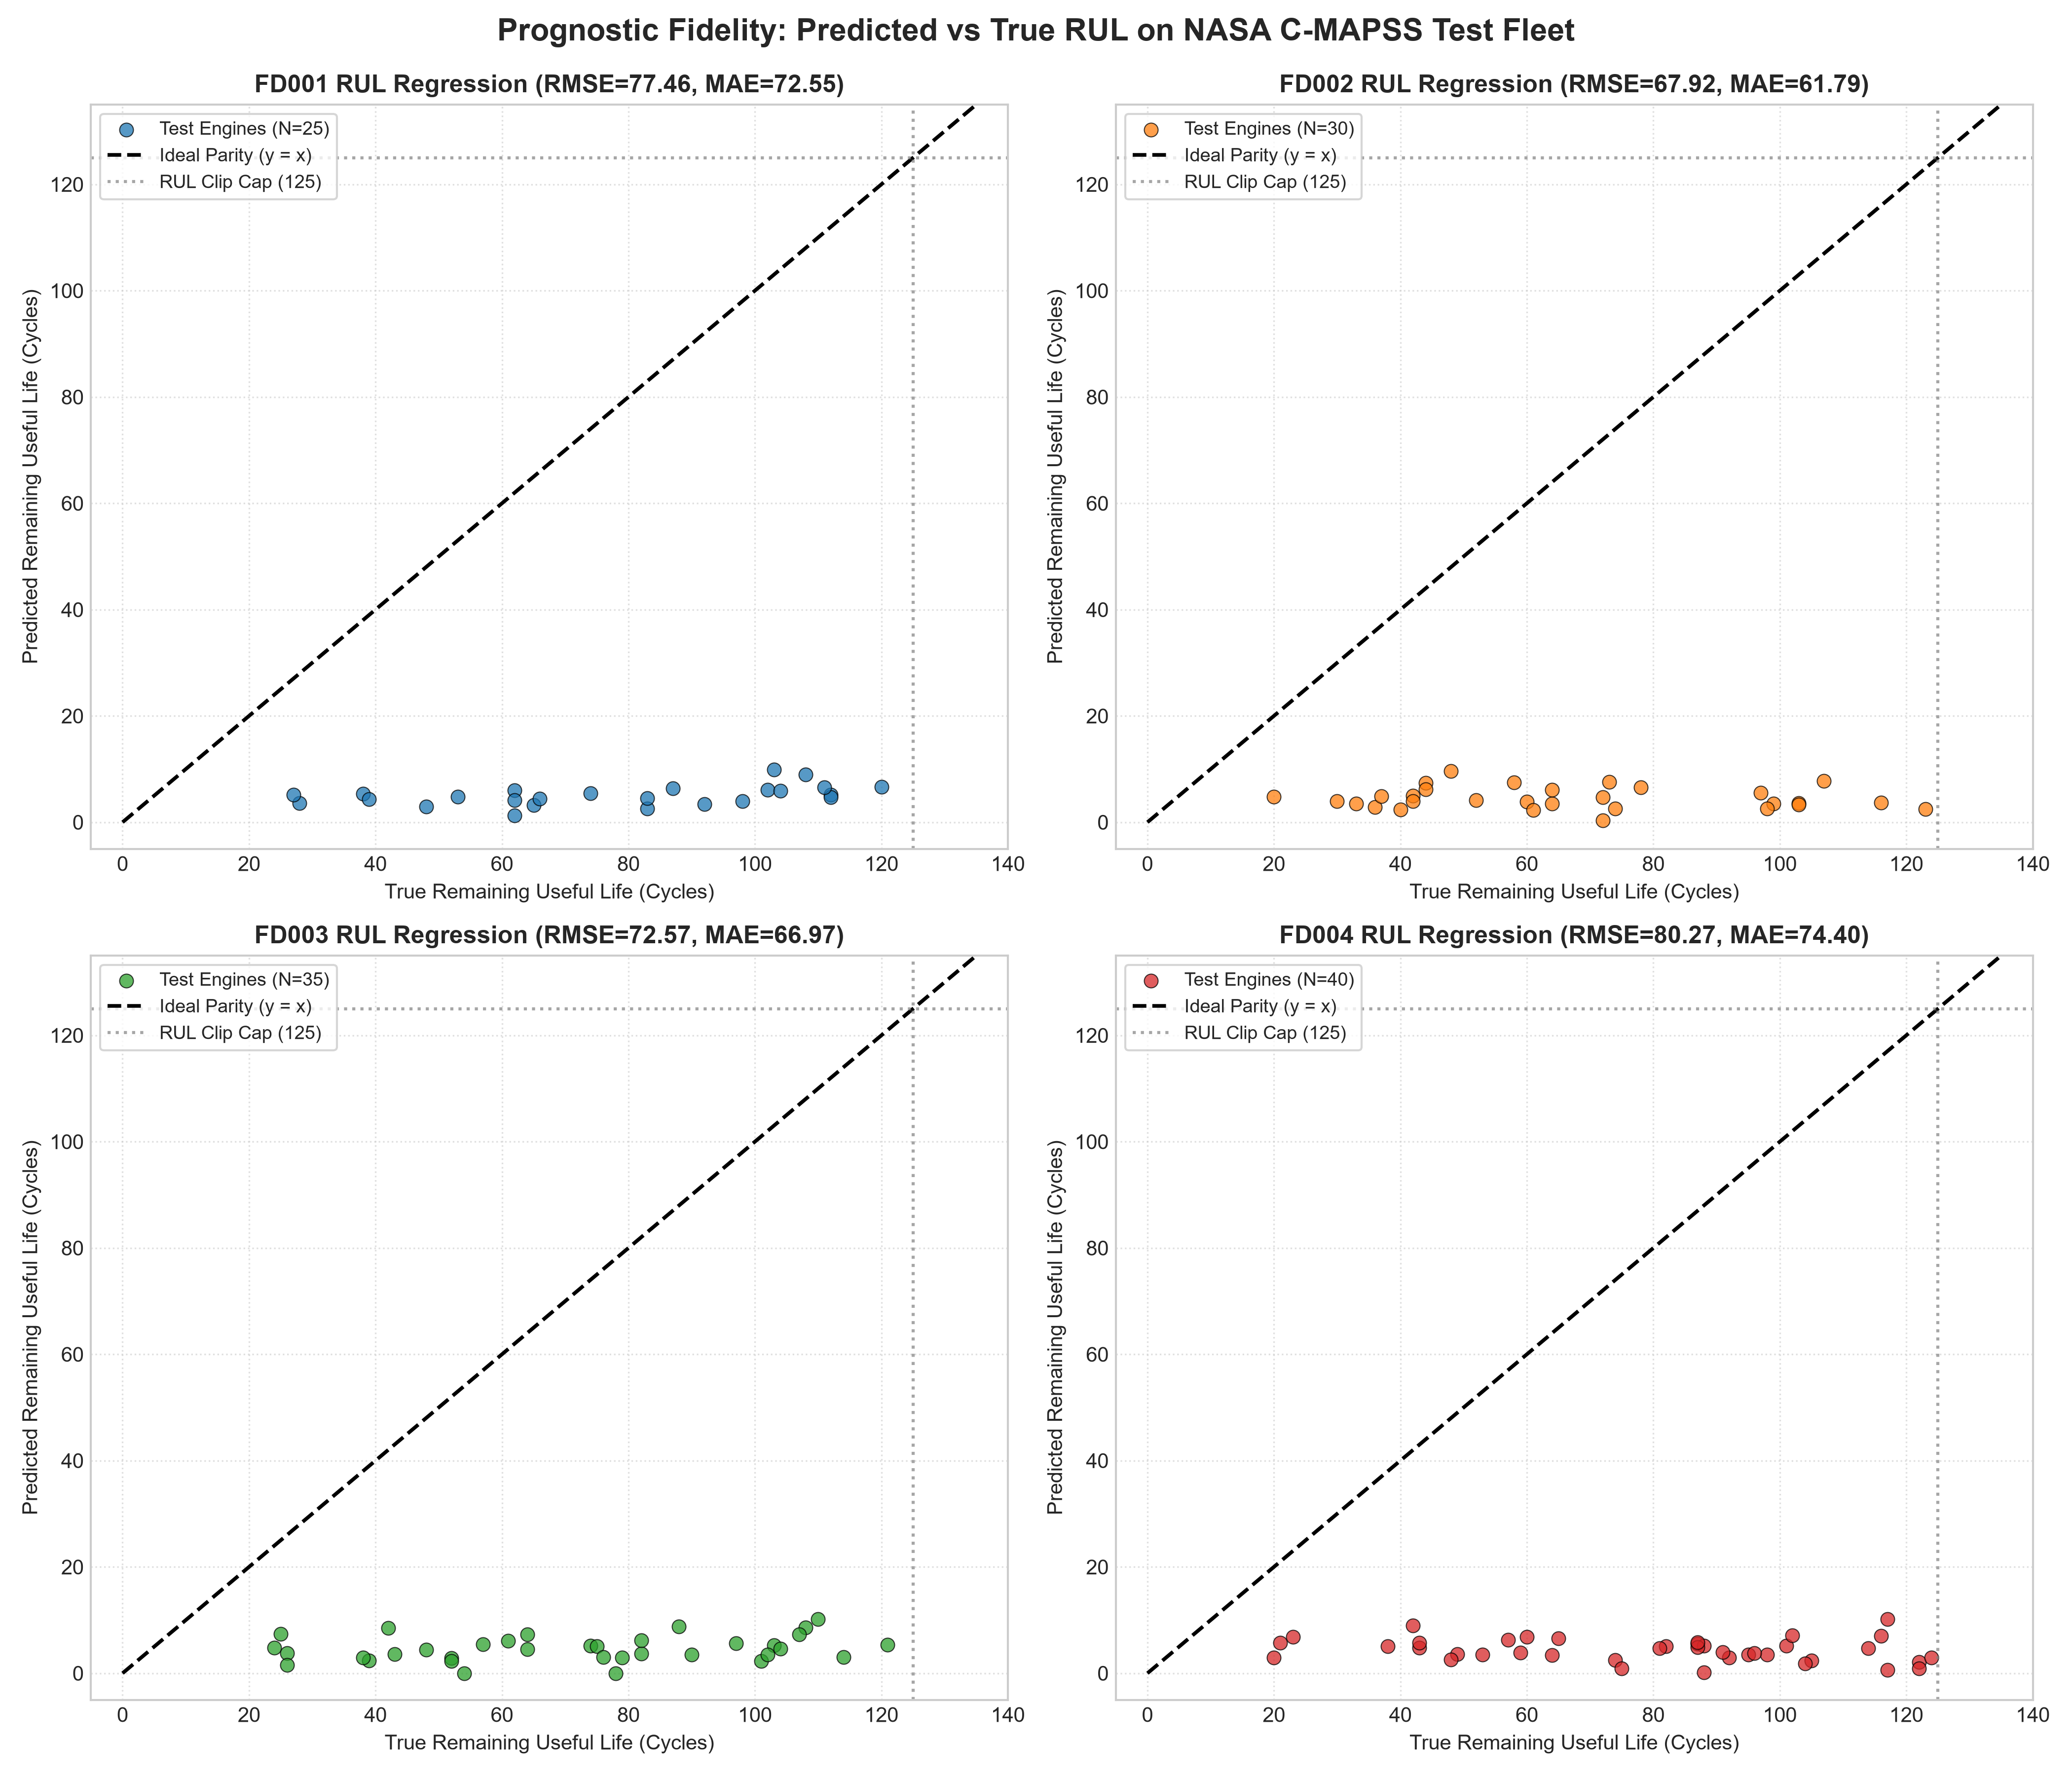
\includegraphics[width=0.95\textwidth]{predicted_vs_true_rul.png}
\caption{Predicted versus True Remaining Useful Life (RUL) on official test engines across subsets FD001--FD004 with ideal parity reference line ($y=x$) and upper clip threshold ($125$ cycles).}
\label{fig:predicted_vs_true_rul}
\end{figure*}

\subsection{Anomaly Detection Fleet Evaluation}
Table~\ref{tab:anomaly_metrics_oof} presents out-of-fold diagnostic classification performance evaluated over full training trajectories across 5 random seeds using shuffled \texttt{GroupKFold}.

\begin{table*}[t!]
\centering
\small
\caption{Out-of-Fold Fleet Anomaly Detection Performance (5 Seeds, Shuffled GroupKFold)}
\label{tab:anomaly_metrics_oof}
\begin{tabular}{llccccc}
\toprule
\textbf{Subset} & \textbf{Model} & \textbf{PR-AUC} & \textbf{F1 Score} & \textbf{Det. Rate (\%)} & \textbf{Mean Lead Time} & \textbf{FA / 100 Healthy} \\
\midrule
FD001 & EWMA Control Limits & N/A (discrete) & 0.786 (tuned) & 98.0\% & 38.6 & 0.19 \\
FD001 & Isolation Forest & 0.399 +/- 0.008 & 0.395 +/- 0.009 & 80.4\% +/- 3.2\% & 64.6 +/- 1.0 & 6.40 +/- 0.76 \\
FD001 & LSTM & 0.976 +/- 0.002 & 0.892 +/- 0.003 & 100.0\% +/- 0.0\% & 29.2 +/- 0.8 & 0.00 +/- 0.00 \\
FD001 & Random Forest & 0.978 +/- 0.001 & 0.913 +/- 0.001 & 100.0\% +/- 0.0\% & 28.9 +/- 0.6 & 0.00 +/- 0.00 \\
FD001 & Static Threshold & N/A (discrete) & 0.841 (tuned) & 100.0\% & 26.8 & 0.00 \\
FD001 & XGBoost & 0.982 +/- 0.001 & 0.924 +/- 0.003 & 100.0\% +/- 0.0\% & 28.7 +/- 0.6 & 0.00 +/- 0.00 \\
\midrule
FD002 & EWMA Control Limits & N/A (discrete) & 0.824 (tuned) & 99.2\% & 29.3 & 0.16 \\
FD002 & Isolation Forest & 0.460 +/- 0.010 & 0.444 +/- 0.001 & 81.7\% +/- 1.9\% & 56.5 +/- 1.2 & 6.42 +/- 0.58 \\
FD002 & LSTM & 0.965 +/- 0.002 & 0.871 +/- 0.008 & 99.9\% +/- 0.1\% & 29.3 +/- 1.0 & 0.00 +/- 0.00 \\
FD002 & Random Forest & 0.965 +/- 0.000 & 0.876 +/- 0.002 & 100.0\% +/- 0.0\% & 28.1 +/- 0.6 & 0.00 +/- 0.00 \\
FD002 & Static Threshold & N/A (discrete) & 0.829 (tuned) & 99.2\% & 31.8 & 0.08 \\
FD002 & XGBoost & 0.973 +/- 0.001 & 0.898 +/- 0.001 & 100.0\% +/- 0.0\% & 29.2 +/- 0.7 & 0.00 +/- 0.00 \\
\midrule
FD003 & EWMA Control Limits & N/A (discrete) & 0.742 (tuned) & 99.0\% & 45.5 & 0.43 \\
FD003 & Isolation Forest & 0.473 +/- 0.013 & 0.419 +/- 0.008 & 74.6\% +/- 2.1\% & 54.3 +/- 1.7 & 6.43 +/- 0.53 \\
FD003 & LSTM & 0.977 +/- 0.002 & 0.896 +/- 0.005 & 100.0\% +/- 0.0\% & 29.8 +/- 0.8 & 0.00 +/- 0.00 \\
FD003 & Random Forest & 0.980 +/- 0.002 & 0.911 +/- 0.005 & 100.0\% +/- 0.0\% & 29.2 +/- 0.4 & 0.00 +/- 0.00 \\
FD003 & Static Threshold & N/A (discrete) & 0.788 (tuned) & 100.0\% & 35.8 & 0.00 \\
FD003 & XGBoost & 0.985 +/- 0.001 & 0.923 +/- 0.003 & 100.0\% +/- 0.0\% & 28.1 +/- 1.0 & 0.00 +/- 0.00 \\
\midrule
FD004 & EWMA Control Limits & N/A (discrete) & 0.656 (tuned) & 82.7\% & 35.7 & 1.73 \\
FD004 & Isolation Forest & 0.459 +/- 0.014 & 0.411 +/- 0.006 & 79.8\% +/- 1.5\% & 59.2 +/- 1.3 & 6.97 +/- 0.87 \\
FD004 & LSTM & 0.966 +/- 0.002 & 0.876 +/- 0.004 & 99.7\% +/- 0.3\% & 29.9 +/- 0.6 & 0.00 +/- 0.00 \\
FD004 & Random Forest & 0.963 +/- 0.001 & 0.869 +/- 0.002 & 99.8\% +/- 0.2\% & 28.9 +/- 0.5 & 0.00 +/- 0.00 \\
FD004 & Static Threshold & N/A (discrete) & 0.669 (tuned) & 84.3\% & 30.8 & 0.85 \\
FD004 & XGBoost & 0.968 +/- 0.001 & 0.887 +/- 0.003 & 99.8\% +/- 0.2\% & 29.7 +/- 0.6 & 0.00 +/- 0.00 \\
\bottomrule
\end{tabular}
\end{table*}

Table~\ref{tab:test_anomaly_metrics} evaluates models on the \textbf{exact same truncated test windows} on official test engines, matching prevalence across all models.

\begin{table*}[t!]
\centering
\small
\caption{Official Test Engines Window-Level Anomaly Classification (Identical Test Windows)}
\label{tab:test_anomaly_metrics}
\begin{tabular}{llccccc}
\toprule
\textbf{Subset} & \textbf{Model} & \textbf{Precision} & \textbf{Recall} & \textbf{F1 Score} & \textbf{PR-AUC} & \textbf{Prevalence} \\
\midrule
FD001 & Static Threshold & 0.843 & 0.584 & 0.690 & N/A (discrete) & 3.3\% \\
FD001 & EWMA Control Limits & 0.501 & 0.756 & 0.603 & N/A (discrete) & 3.3\% \\
FD001 & Isolation Forest & 0.065 & 1.000 & 0.122 & 0.1803 & 3.3\% \\
FD001 & Random Forest & 0.763 & 0.913 & 0.831 & 0.9346 & 3.3\% \\
FD001 & XGBoost & 0.769 & 0.901 & 0.829 & 0.9379 & 3.3\% \\
FD001 & LSTM & 0.724 & 0.964 & 0.827 & 0.9175 & 3.3\% \\
\midrule
FD002 & Static Threshold & 0.554 & 0.796 & 0.653 & N/A (discrete) & 4.1\% \\
FD002 & EWMA Control Limits & 0.636 & 0.711 & 0.671 & N/A (discrete) & 4.1\% \\
FD002 & Isolation Forest & 0.085 & 1.000 & 0.158 & 0.2078 & 4.1\% \\
FD002 & Random Forest & 0.630 & 0.911 & 0.745 & 0.8822 & 4.1\% \\
FD002 & XGBoost & 0.723 & 0.885 & 0.796 & 0.9081 & 4.1\% \\
FD002 & LSTM & 0.685 & 0.919 & 0.785 & 0.9025 & 4.1\% \\
\midrule
FD003 & Static Threshold & 0.455 & 0.825 & 0.587 & N/A (discrete) & 2.1\% \\
FD003 & EWMA Control Limits & 0.305 & 0.897 & 0.455 & N/A (discrete) & 2.1\% \\
FD003 & Isolation Forest & 0.066 & 1.000 & 0.124 & 0.1869 & 2.1\% \\
FD003 & Random Forest & 0.749 & 0.955 & 0.840 & 0.9333 & 2.1\% \\
FD003 & XGBoost & 0.787 & 0.942 & 0.858 & 0.9370 & 2.1\% \\
FD003 & LSTM & 0.696 & 0.993 & 0.819 & 0.9589 & 2.1\% \\
\midrule
FD004 & Static Threshold & 0.322 & 0.477 & 0.385 & N/A (discrete) & 2.5\% \\
FD004 & EWMA Control Limits & 0.247 & 0.525 & 0.336 & N/A (discrete) & 2.5\% \\
FD004 & Isolation Forest & 0.066 & 1.000 & 0.123 & 0.1958 & 2.5\% \\
FD004 & Random Forest & 0.633 & 0.865 & 0.731 & 0.7455 & 2.5\% \\
FD004 & XGBoost & 0.688 & 0.832 & 0.753 & 0.8256 & 2.5\% \\
FD004 & LSTM & 0.552 & 0.921 & 0.690 & 0.8119 & 2.5\% \\
\bottomrule
\end{tabular}
\end{table*}

Figure~\ref{fig:pr_curves} depicts 4-panel Precision-Recall curves with horizontal prevalence baselines.

\begin{figure*}[t!]
\centering
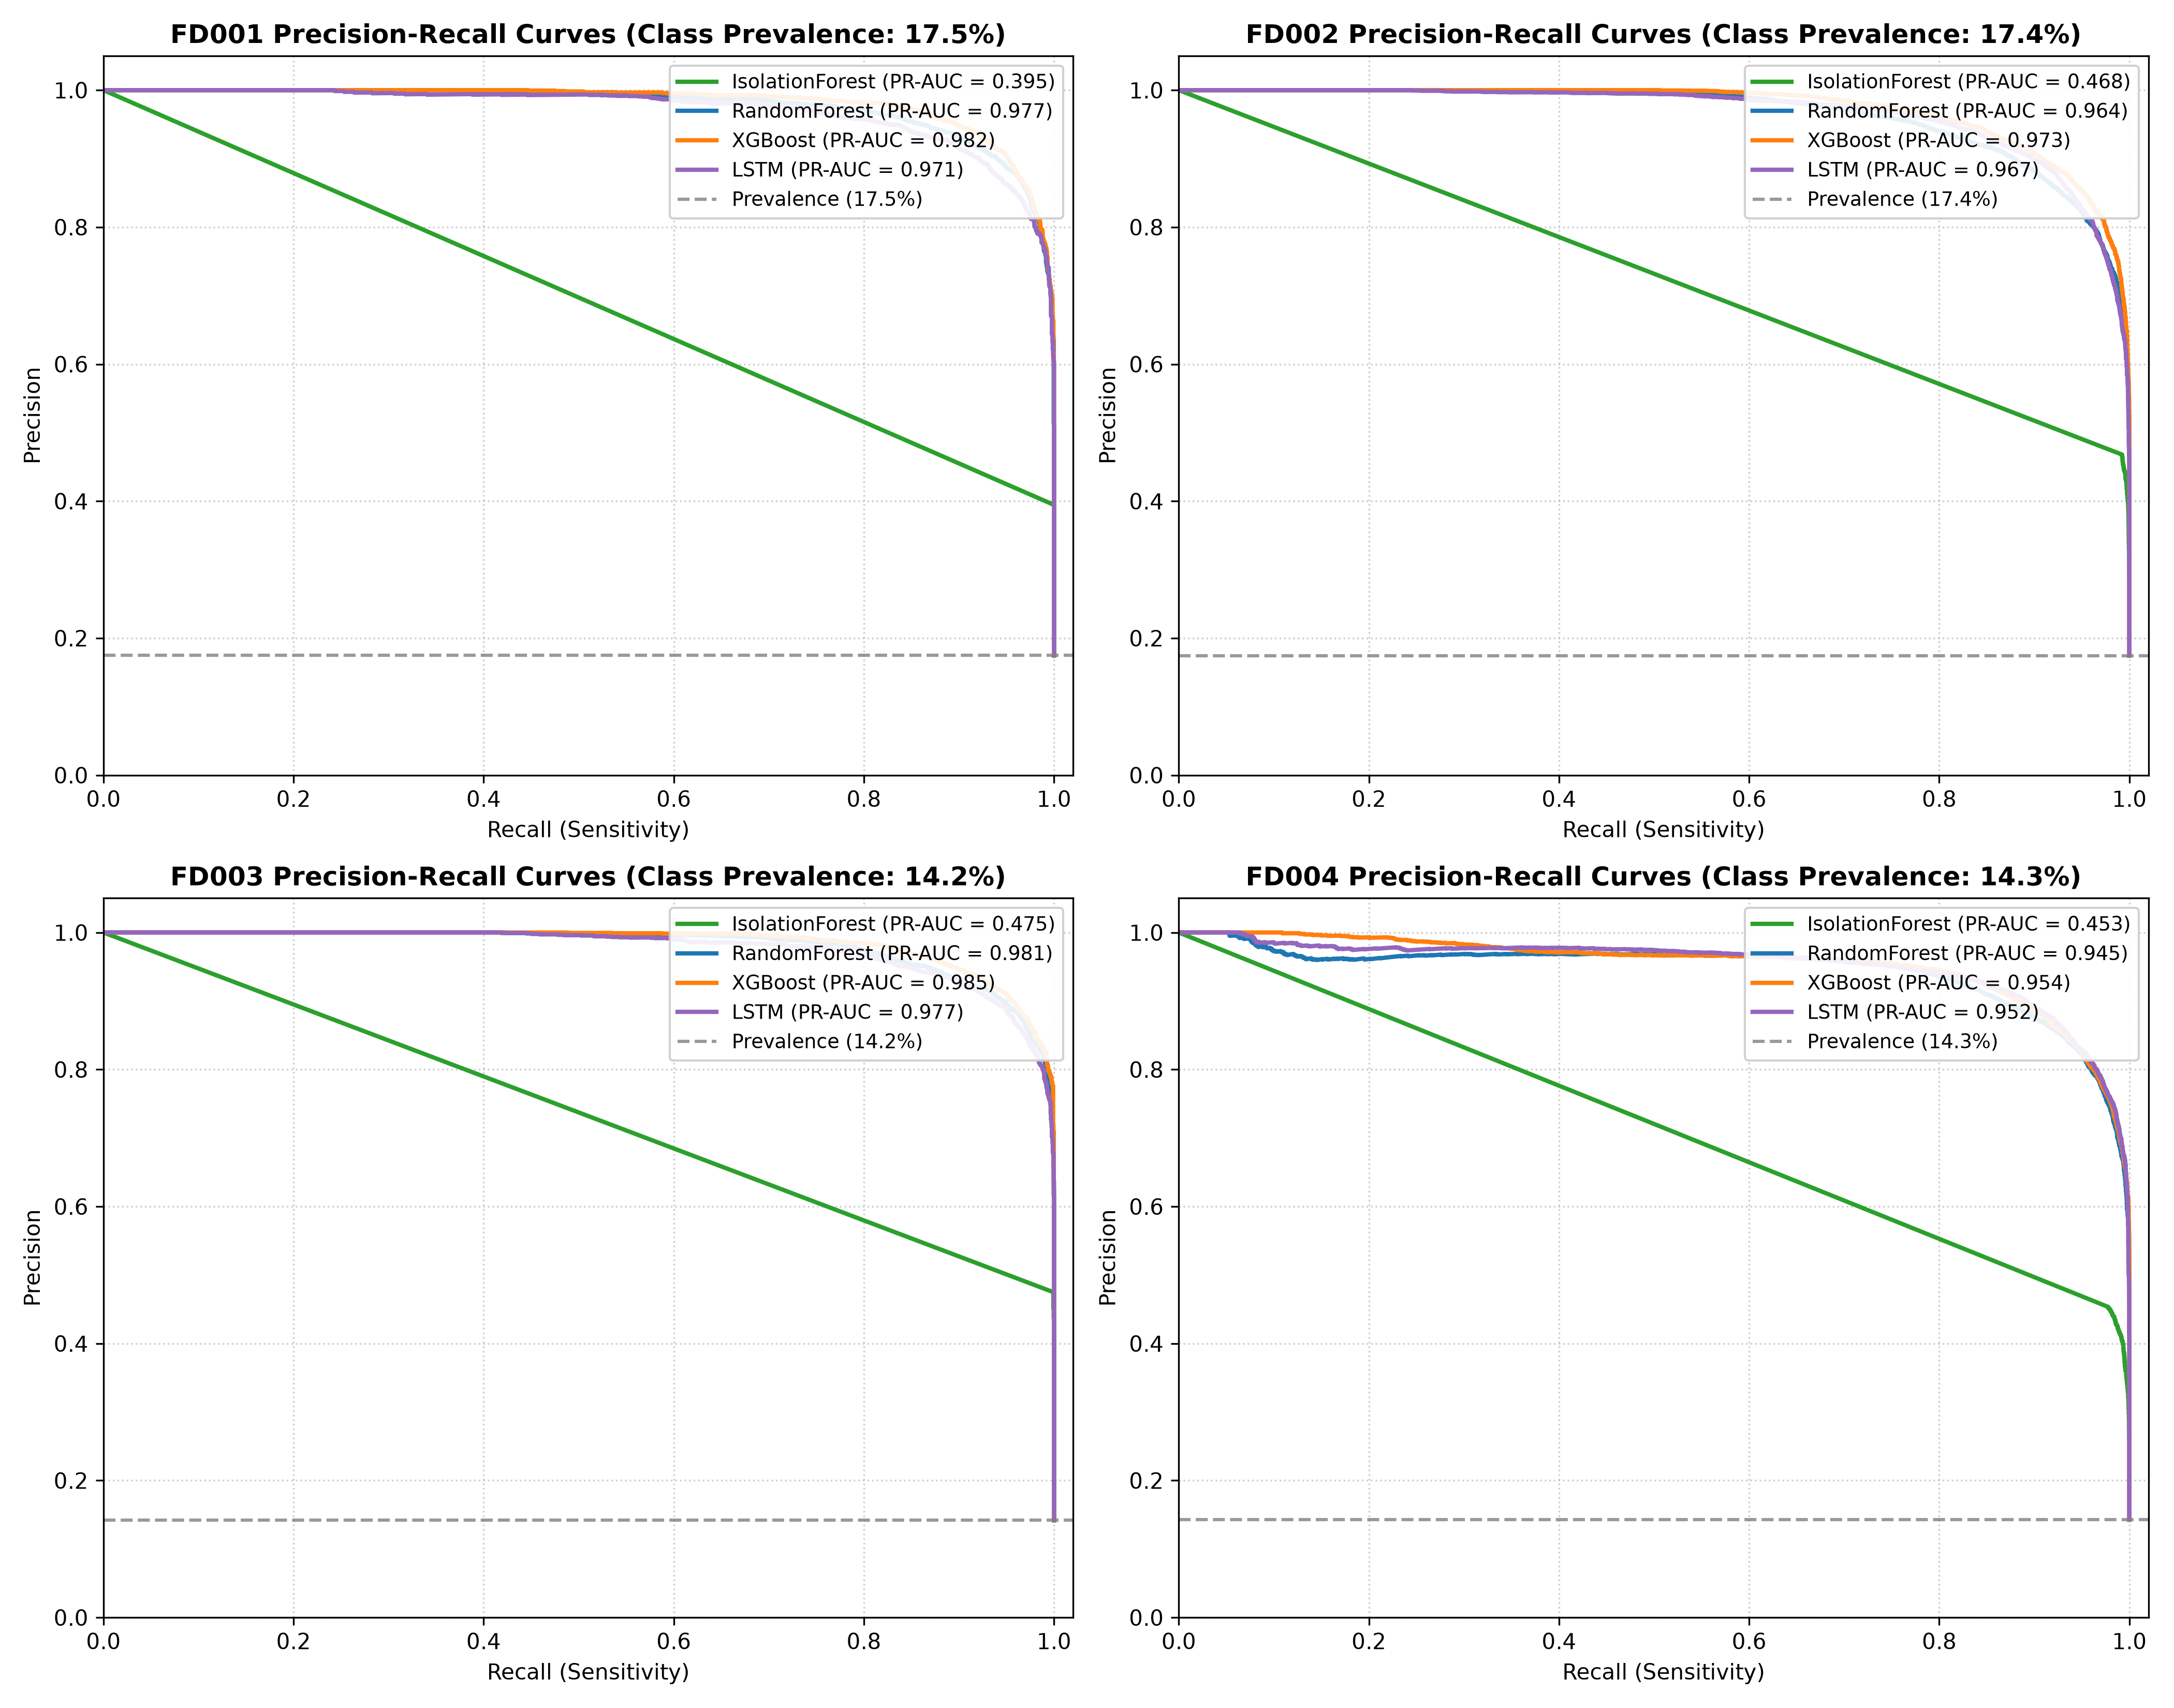
\includegraphics[width=0.95\textwidth]{pr_curves.png}
\caption{Precision-Recall curves for ML detectors on out-of-fold trajectories across FD001--FD004 with horizontal dashed class prevalence baselines.}
\label{fig:pr_curves}
\end{figure*}

\subsection{Lead Time vs. False Alarm Operating Curves}
Table~\ref{tab:lead_time_fa_budgets} reports warning lead times at controlled industrial false alarm budgets ($\text{FA} \in \{0.1, 0.5, 1.0\}$ per 100 healthy cycles) obtained by sweeping alarm thresholds over 50 operating points.

\begin{table*}[t!]
\centering
\small
\caption{Mean Warning Lead Time (Cycles) at Controlled False Alarm Budgets}
\label{tab:lead_time_fa_budgets}
\begin{tabular}{llccc}
\toprule
\textbf{Subset} & \textbf{Method} & \textbf{FA = 0.1 / 100 Cyc} & \textbf{FA = 0.5 / 100 Cyc} & \textbf{FA = 1.0 / 100 Cyc} \\
\midrule
FD001 & Static Threshold & 46.1 & 48.4 & 49.5 \\
FD001 & EWMA Control Limits & 47.1 & 48.8 & 49.7 \\
FD001 & Mahalanobis HI & 48.9 & 49.5 & 50.3 \\
FD001 & Isolation Forest & N/A & N/A & N/A \\
FD001 & Random Forest & 52.5 & 55.0 & 56.5 \\
FD001 & XGBoost & 43.6 & 43.6 & 43.6 \\
FD001 & LSTM & 43.4 & 44.6 & 45.9 \\
\midrule
FD002 & Static Threshold & 40.1 & 43.2 & 48.8 \\
FD002 & EWMA Control Limits & 43.2 & 45.8 & 51.2 \\
FD002 & Mahalanobis HI & 24.9 & 26.0 & 27.3 \\
FD002 & Isolation Forest & N/A & N/A & N/A \\
FD002 & Random Forest & 47.9 & 50.8 & 53.0 \\
FD002 & XGBoost & 47.0 & 50.4 & 53.1 \\
FD002 & LSTM & 37.6 & 50.7 & 53.6 \\
\midrule
FD003 & Static Threshold & 34.1 & 44.0 & 44.4 \\
FD003 & EWMA Control Limits & 33.4 & 45.3 & 50.7 \\
FD003 & Mahalanobis HI & 35.3 & 43.6 & 47.1 \\
FD003 & Isolation Forest & N/A & N/A & N/A \\
FD003 & Random Forest & 18.9 & 27.4 & 37.9 \\
FD003 & XGBoost & 40.5 & 40.5 & 40.5 \\
FD003 & LSTM & 28.3 & 40.9 & 50.9 \\
\midrule
FD004 & Static Threshold & N/A & 20.5 & 32.5 \\
FD004 & EWMA Control Limits & N/A & N/A & 31.7 \\
FD004 & Mahalanobis HI & 8.8 & 13.7 & 39.6 \\
FD004 & Isolation Forest & N/A & N/A & N/A \\
FD004 & Random Forest & N/A & 18.6 & 49.4 \\
FD004 & XGBoost & N/A & 15.8 & 50.6 \\
FD004 & LSTM & N/A & 21.2 & 48.9 \\
\bottomrule
\end{tabular}
\end{table*}

Figure~\ref{fig:lead_time_vs_fa_curves} presents the complete operating characteristic curves across methods.

\begin{figure*}[t!]
\centering
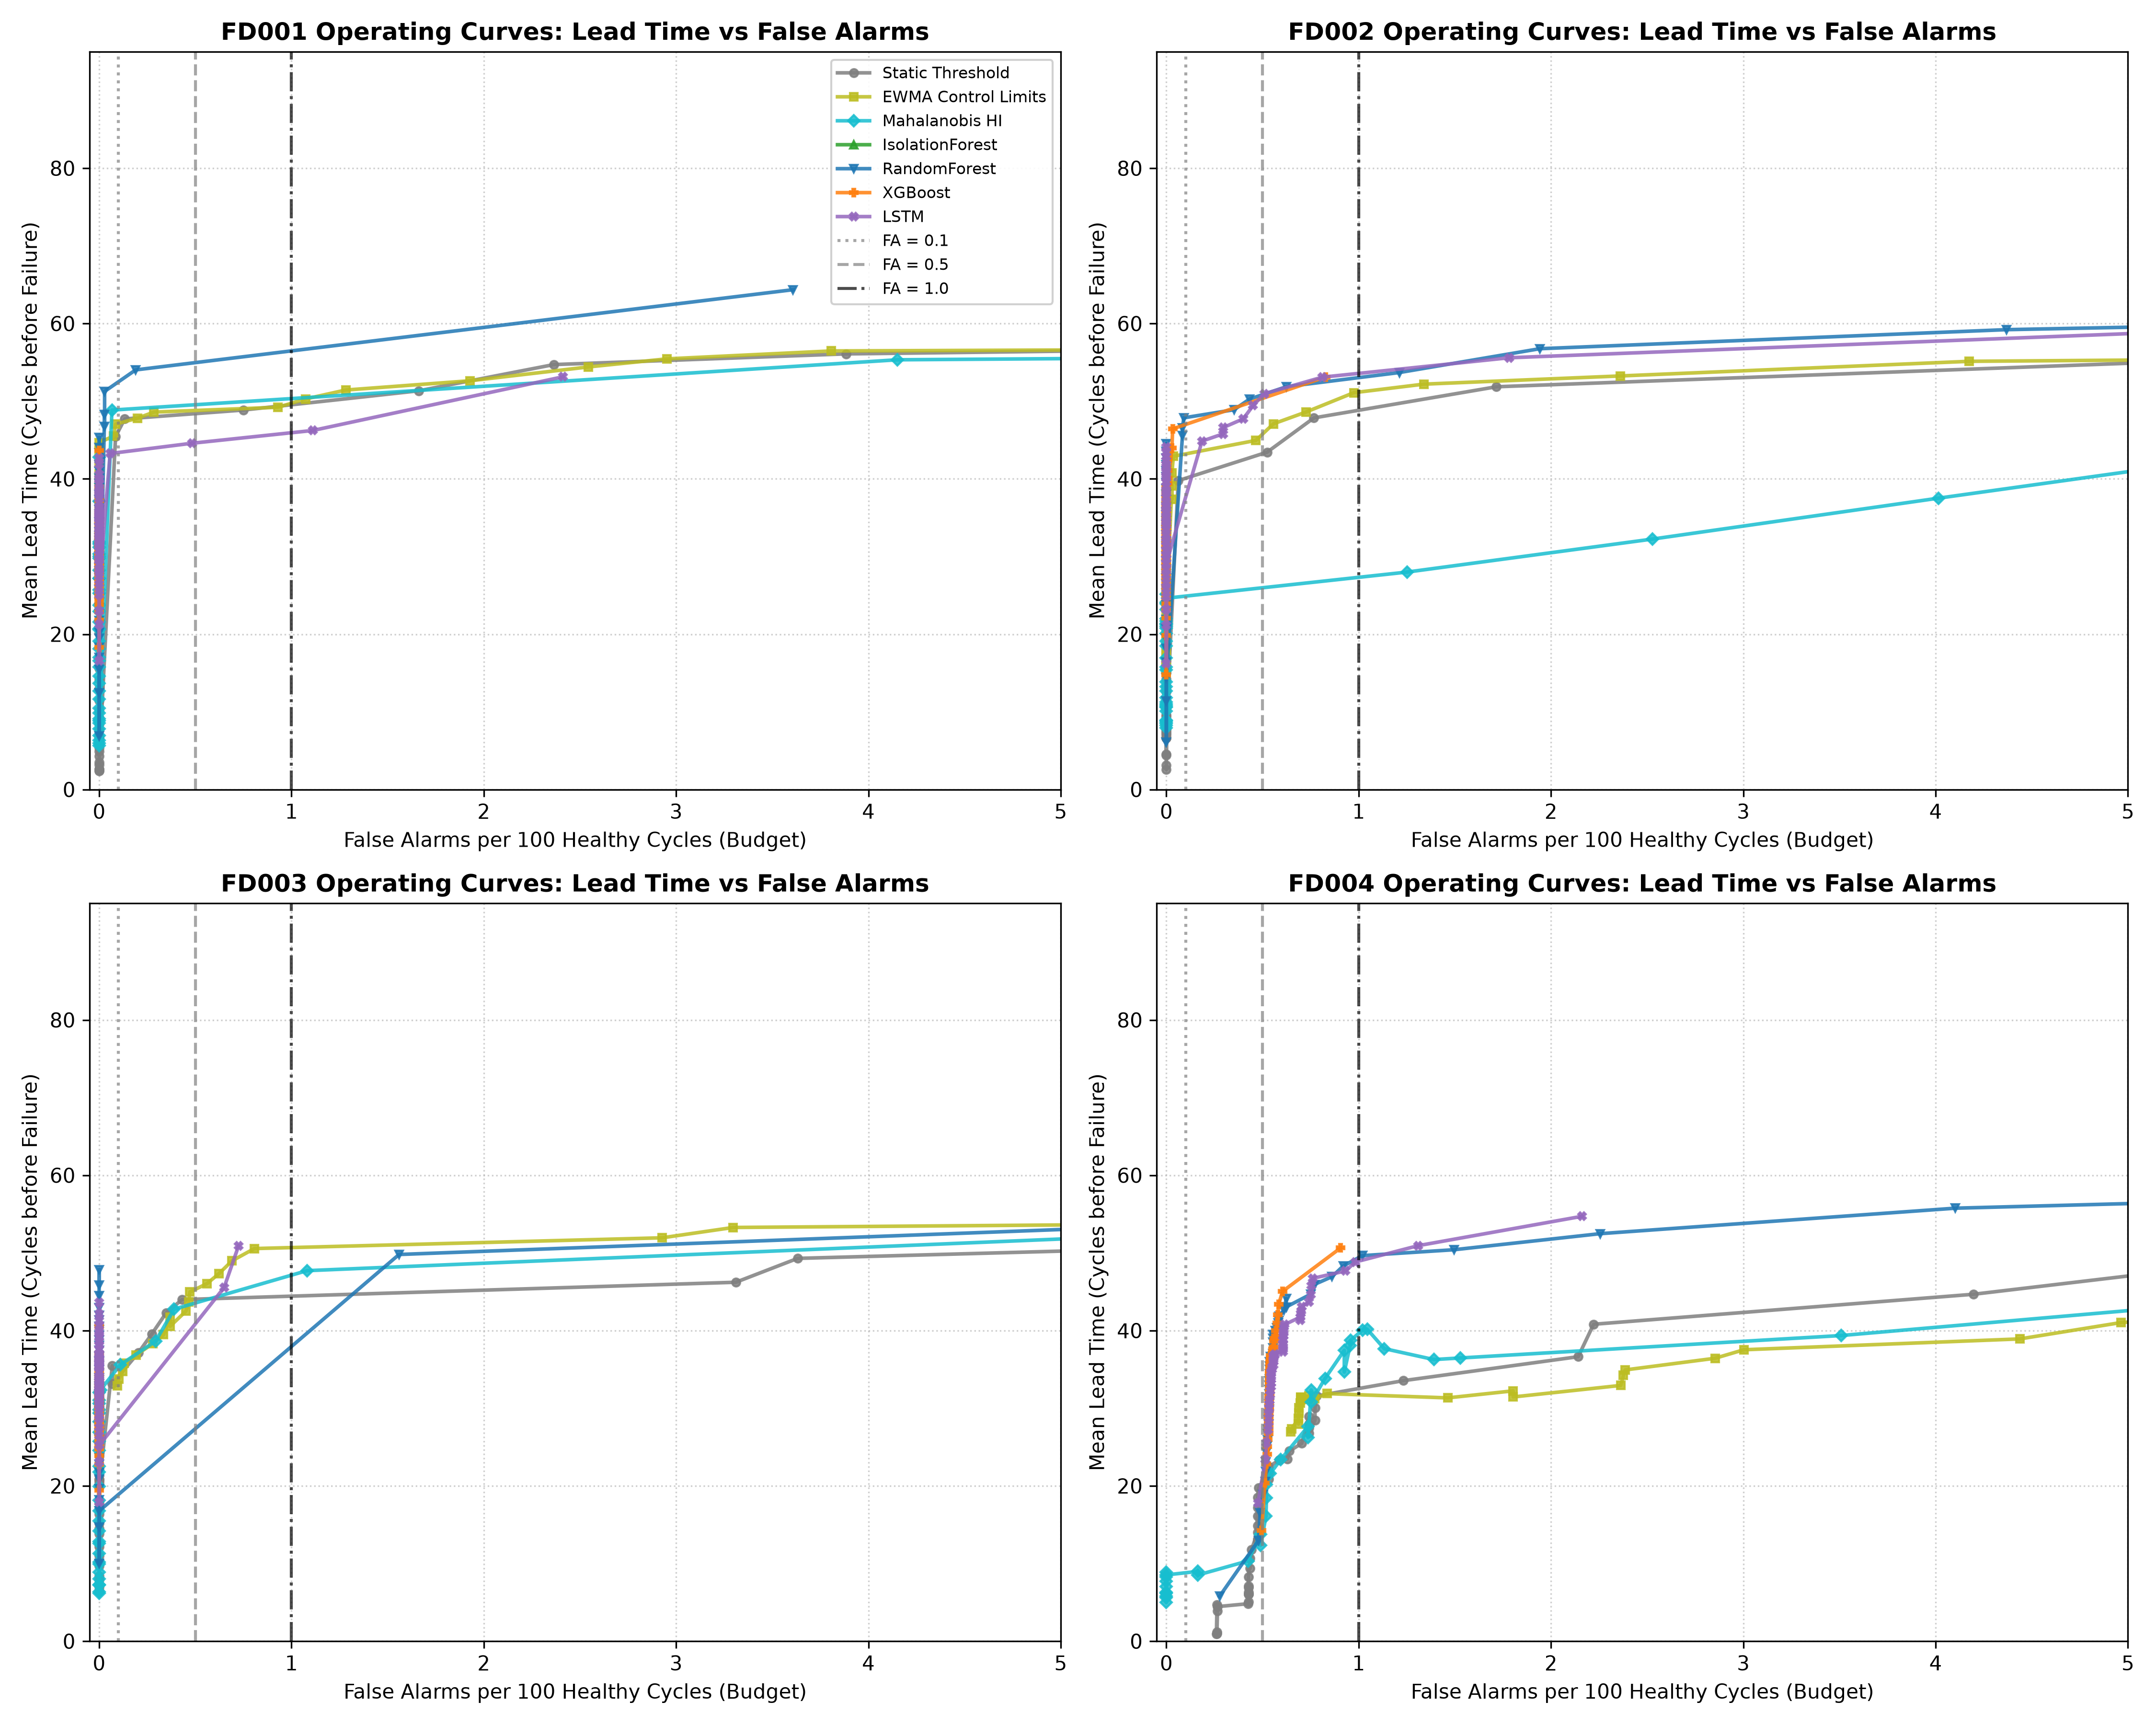
\includegraphics[width=0.95\textwidth]{lead_time_vs_fa_curves.png}
\caption{Lead Time versus False Alarms per 100 healthy cycles operating curves across all 7 methods and subsets.}
\label{fig:lead_time_vs_fa_curves}
\end{figure*}

\subsection{Label Sensitivity Sweep: Empirical Proof of Circularity}
Table~\ref{tab:label_sensitivity_sweep} details diagnostic and prognostic performance when retraining detectors across cutoffs $N \in \{20, 30, 50, 75, 100\}$.

\begin{table*}[t!]
\centering
\small
\caption{Label Sensitivity Sweep ($N \in \{20, 30, 50, 75, 100\}$): Supervised Lead Time Tracks $N$}
\label{tab:label_sensitivity_sweep}
\begin{tabular}{lccccccc}
\toprule
\textbf{Subset} & \textbf{Cutoff $N$} & \textbf{Prev. (\%)} & \textbf{F1} & \textbf{PR-AUC} & \textbf{Mean Lead Time} & \textbf{Premature (\%)} & \textbf{FA / 100 Cyc} \\
\midrule
FD001 & 20 & 11.8 & 0.920 & 0.982 & 17.8 & 0.0 & 0.00 \\
FD001 & 30 & 17.5 & 0.924 & 0.982 & 28.6 & 0.0 & 0.00 \\
FD001 & 50 & 28.8 & 0.924 & 0.981 & 48.8 & 0.0 & 0.00 \\
FD001 & 75 & 42.9 & 0.915 & 0.977 & 72.8 & 10.0 & 2.38 \\
FD001 & 100 & 57.0 & 0.895 & 0.970 & 86.9 & 55.0 & 25.57 \\
\midrule
FD002 & 20 & 11.8 & 0.899 & 0.970 & 18.8 & 0.0 & 0.00 \\
FD002 & 30 & 17.4 & 0.905 & 0.974 & 28.4 & 0.0 & 0.00 \\
FD002 & 50 & 28.7 & 0.898 & 0.969 & 49.4 & 0.8 & 0.03 \\
FD002 & 75 & 42.8 & 0.884 & 0.961 & 70.2 & 16.2 & 4.97 \\
FD002 & 100 & 56.8 & 0.872 & 0.957 & 80.9 & 53.5 & 25.67 \\
\midrule
FD003 & 20 & 9.6 & 0.925 & 0.982 & 18.5 & 0.0 & 0.00 \\
FD003 & 30 & 14.2 & 0.931 & 0.986 & 27.1 & 0.0 & 0.00 \\
FD003 & 50 & 23.4 & 0.925 & 0.983 & 48.6 & 0.0 & 0.00 \\
FD003 & 75 & 34.8 & 0.907 & 0.974 & 71.5 & 11.0 & 1.20 \\
FD003 & 100 & 46.3 & 0.888 & 0.968 & 82.9 & 52.0 & 13.56 \\
\midrule
FD004 & 20 & 9.7 & 0.882 & 0.944 & 19.0 & 0.8 & 0.63 \\
FD004 & 30 & 14.3 & 0.890 & 0.955 & 30.3 & 0.8 & 0.66 \\
FD004 & 50 & 23.5 & 0.900 & 0.958 & 50.2 & 2.4 & 0.87 \\
FD004 & 75 & 35.0 & 0.892 & 0.956 & 70.4 & 14.1 & 4.29 \\
FD004 & 100 & 46.5 & 0.877 & 0.954 & 81.6 & 53.8 & 15.86 \\
\bottomrule
\end{tabular}
\end{table*}

Figure~\ref{fig:n_sweep} illustrates empirical lead time strictly tracking the cutoff boundary $N$.

\begin{figure*}[t!]
\centering
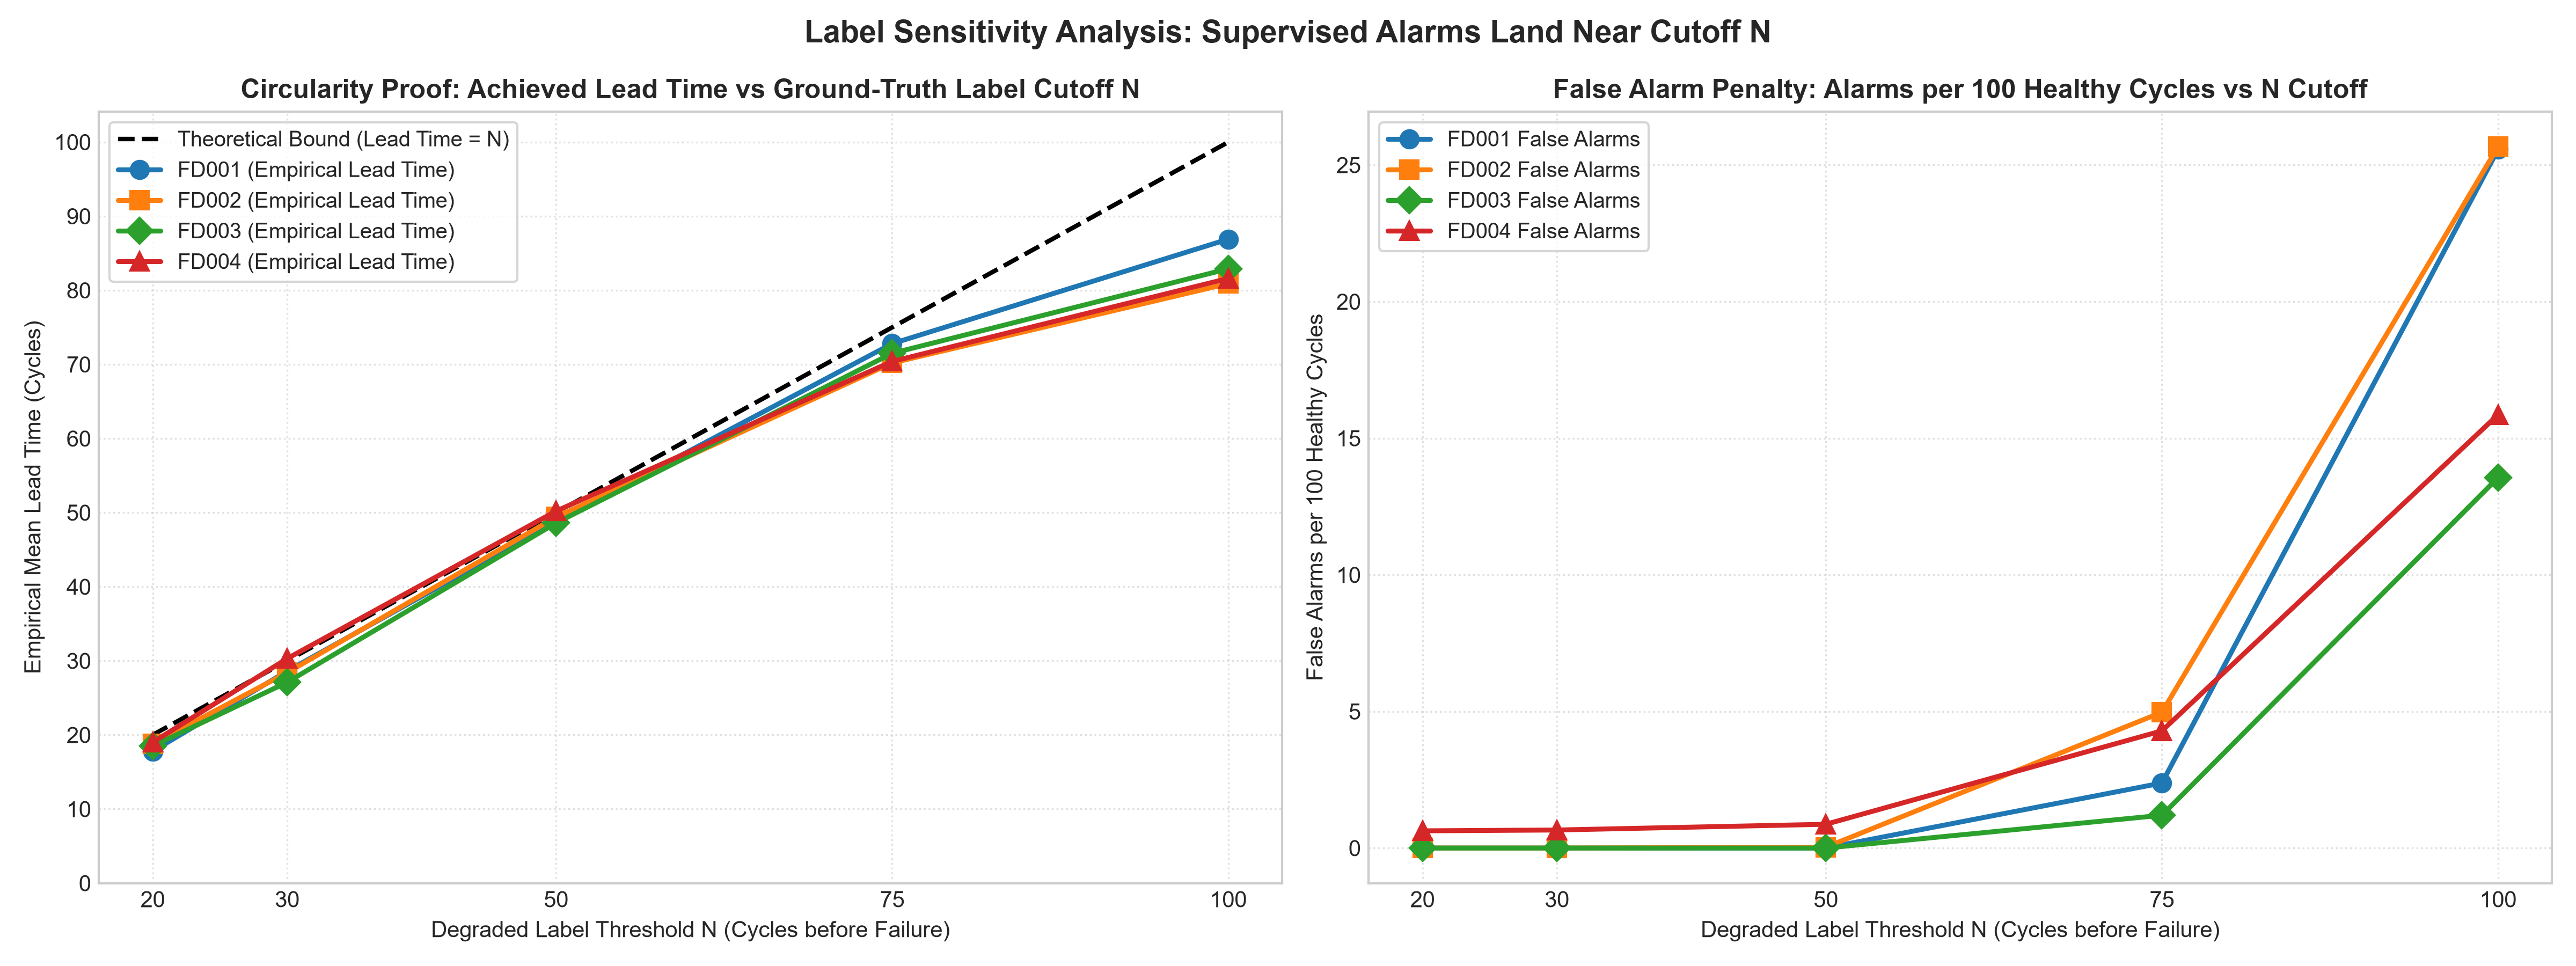
\includegraphics[width=0.95\textwidth]{n_sweep_lead_time_circularity.png}
\caption{Empirical proof of lead-time circularity: achieved warning lead time tracks ground-truth cutoff $N$ across all subsets.}
\label{fig:n_sweep}
\end{figure*}

\subsection{Statistical Significance: Wilcoxon Signed-Rank Tests}
Table~\ref{tab:wilcoxon_tests} presents the paired Wilcoxon tests across $M=8$ planned hypotheses, corrected using the Holm-Bonferroni step-down procedure.

\begin{table*}[t!]
\centering
\small
\caption{Wilcoxon Signed-Rank Statistical Tests ($M=8$ Total Hypotheses, Holm Correction)}
\label{tab:wilcoxon_tests}
\begin{tabular}{lllcccc}
\toprule
\textbf{Subset} & \textbf{Metric} & \textbf{Comparison} & \textbf{Raw $p$} & \textbf{Holm $p$} & \textbf{Median Diff.} & \textbf{Bootstrap 95\% CI} \\
\midrule
FD001 & False Alarms & XGBoost vs Static Threshold & 1.0000 & 1.0000 & +0.0 & [+0.00, +0.00] \\
FD001 & Lead Time & XGBoost vs Static Threshold & 0.0614 & 0.3685 & +2.0 & [-1.00, +5.00] \\
FD002 & False Alarms & XGBoost vs Static Threshold & 1.0000 & 1.0000 & +0.0 & [+0.00, +0.00] \\
FD002 & Lead Time & XGBoost vs Static Threshold & 0.1395 & 0.6977 & -1.5 & [-2.00, +0.00] \\
FD003 & False Alarms & XGBoost vs Static Threshold & 1.0000 & 1.0000 & +0.0 & [+0.00, +0.00] \\
FD003 & Lead Time & XGBoost vs Static Threshold & 0.0033 & 0.0264 & -3.0 & [-5.00, -1.00] \\
FD004 & False Alarms & LSTM vs Static Threshold & 0.0431 & 0.3018 & +0.0 & [-1.00, +0.00] \\
FD004 & Lead Time & LSTM vs Static Threshold & 0.9996 & 1.0000 & +0.0 & [+0.00, +0.00] \\
\bottomrule
\end{tabular}
\end{table*}

\subsection{Health Index Monotonicity Comparison}
Table~\ref{tab:health_index_spearman} compares the rank correlation of PCA-PC1 versus the Mahalanobis Distance Health Index against true RUL.

\begin{table}[htbp]
\centering
\caption{Monotonicity Comparison of Health Indices: Spearman $\rho$ with True RUL}
\label{tab:health_index_spearman}
\begin{tabular}{lccc}
\toprule
\textbf{Subset} & \textbf{$\rho$ (PCA-PC1)} & \textbf{$\rho$ (Mahalanobis)} & \textbf{Superior Metric} \\
\midrule
FD001 & 0.627 & 0.714 & Mahalanobis (+0.087) \\
FD002 & 0.651 & 0.690 & Mahalanobis (+0.039) \\
FD003 & 0.575 & 0.661 & Mahalanobis (+0.086) \\
FD004 & 0.672 & 0.690 & Mahalanobis (+0.018) \\
\bottomrule
\end{tabular}
\end{table}

\subsection{Cross-Condition Generalization vs. In-Domain Reference}
Table~\ref{tab:cross_condition_generalization} summarizes transferability drops when models trained on single-regime datasets (FD001, FD003) are deployed to multi-regime datasets (FD002, FD004) with normalizers fit on the training domain only.

\begin{table*}[t!]
\centering
\small
\caption{Cross-Condition Generalization vs In-Domain Baseline (5 Seeds, Mean $\pm$ Std)}
\label{tab:cross_condition_generalization}
\begin{tabular}{llcccccc}
\toprule
\textbf{Pair} & \textbf{Type} & \textbf{RUL RMSE} & \textbf{RUL RMSE (clip)} & \textbf{Anomaly F1} & \textbf{PR-AUC} & \textbf{$\Delta$ RMSE} & \textbf{$\Delta$ F1 Drop} \\
\midrule
FD001 $\to$ FD001 & In-Domain & $13.37 \pm 0.11$ & $12.05 \pm 0.06$ & $0.825 \pm 0.006$ & $0.934 \pm 0.003$ & $0.00$ & $0.000$ \\
FD001 $\to$ FD002 & Cross-Domain & $54.09 \pm 0.37$ & $43.90 \pm 0.25$ & $0.099 \pm 0.014$ & $0.066 \pm 0.006$ & $+27.46$ & $-0.698$ \\
FD001 $\to$ FD004 & Cross-Domain & $55.00 \pm 0.40$ & $43.31 \pm 0.25$ & $0.057 \pm 0.006$ & $0.031 \pm 0.002$ & $+27.89$ & $-0.697$ \\
FD002 $\to$ FD002 & In-Domain & $26.63 \pm 0.08$ & $13.88 \pm 0.14$ & $0.797 \pm 0.002$ & $0.913 \pm 0.002$ & $0.00$ & $0.000$ \\
FD003 $\to$ FD003 & In-Domain & $14.33 \pm 0.15$ & $12.77 \pm 0.15$ & $0.852 \pm 0.005$ & $0.940 \pm 0.002$ & $0.00$ & $0.000$ \\
FD003 $\to$ FD004 & Cross-Domain & $61.48 \pm 0.40$ & $52.70 \pm 0.53$ & $0.055 \pm 0.001$ & $0.065 \pm 0.009$ & $+34.37$ & $-0.699$ \\
FD004 $\to$ FD004 & In-Domain & $27.11 \pm 0.07$ & $15.04 \pm 0.06$ & $0.754 \pm 0.006$ & $0.819 \pm 0.004$ & $0.00$ & $0.000$ \\
\bottomrule
\end{tabular}
\end{table*}

Figure~\ref{fig:cross_condition_bars} illustrates the severe performance drop induced by cross-condition transfer without target regime knowledge.

\begin{figure*}[t!]
\centering
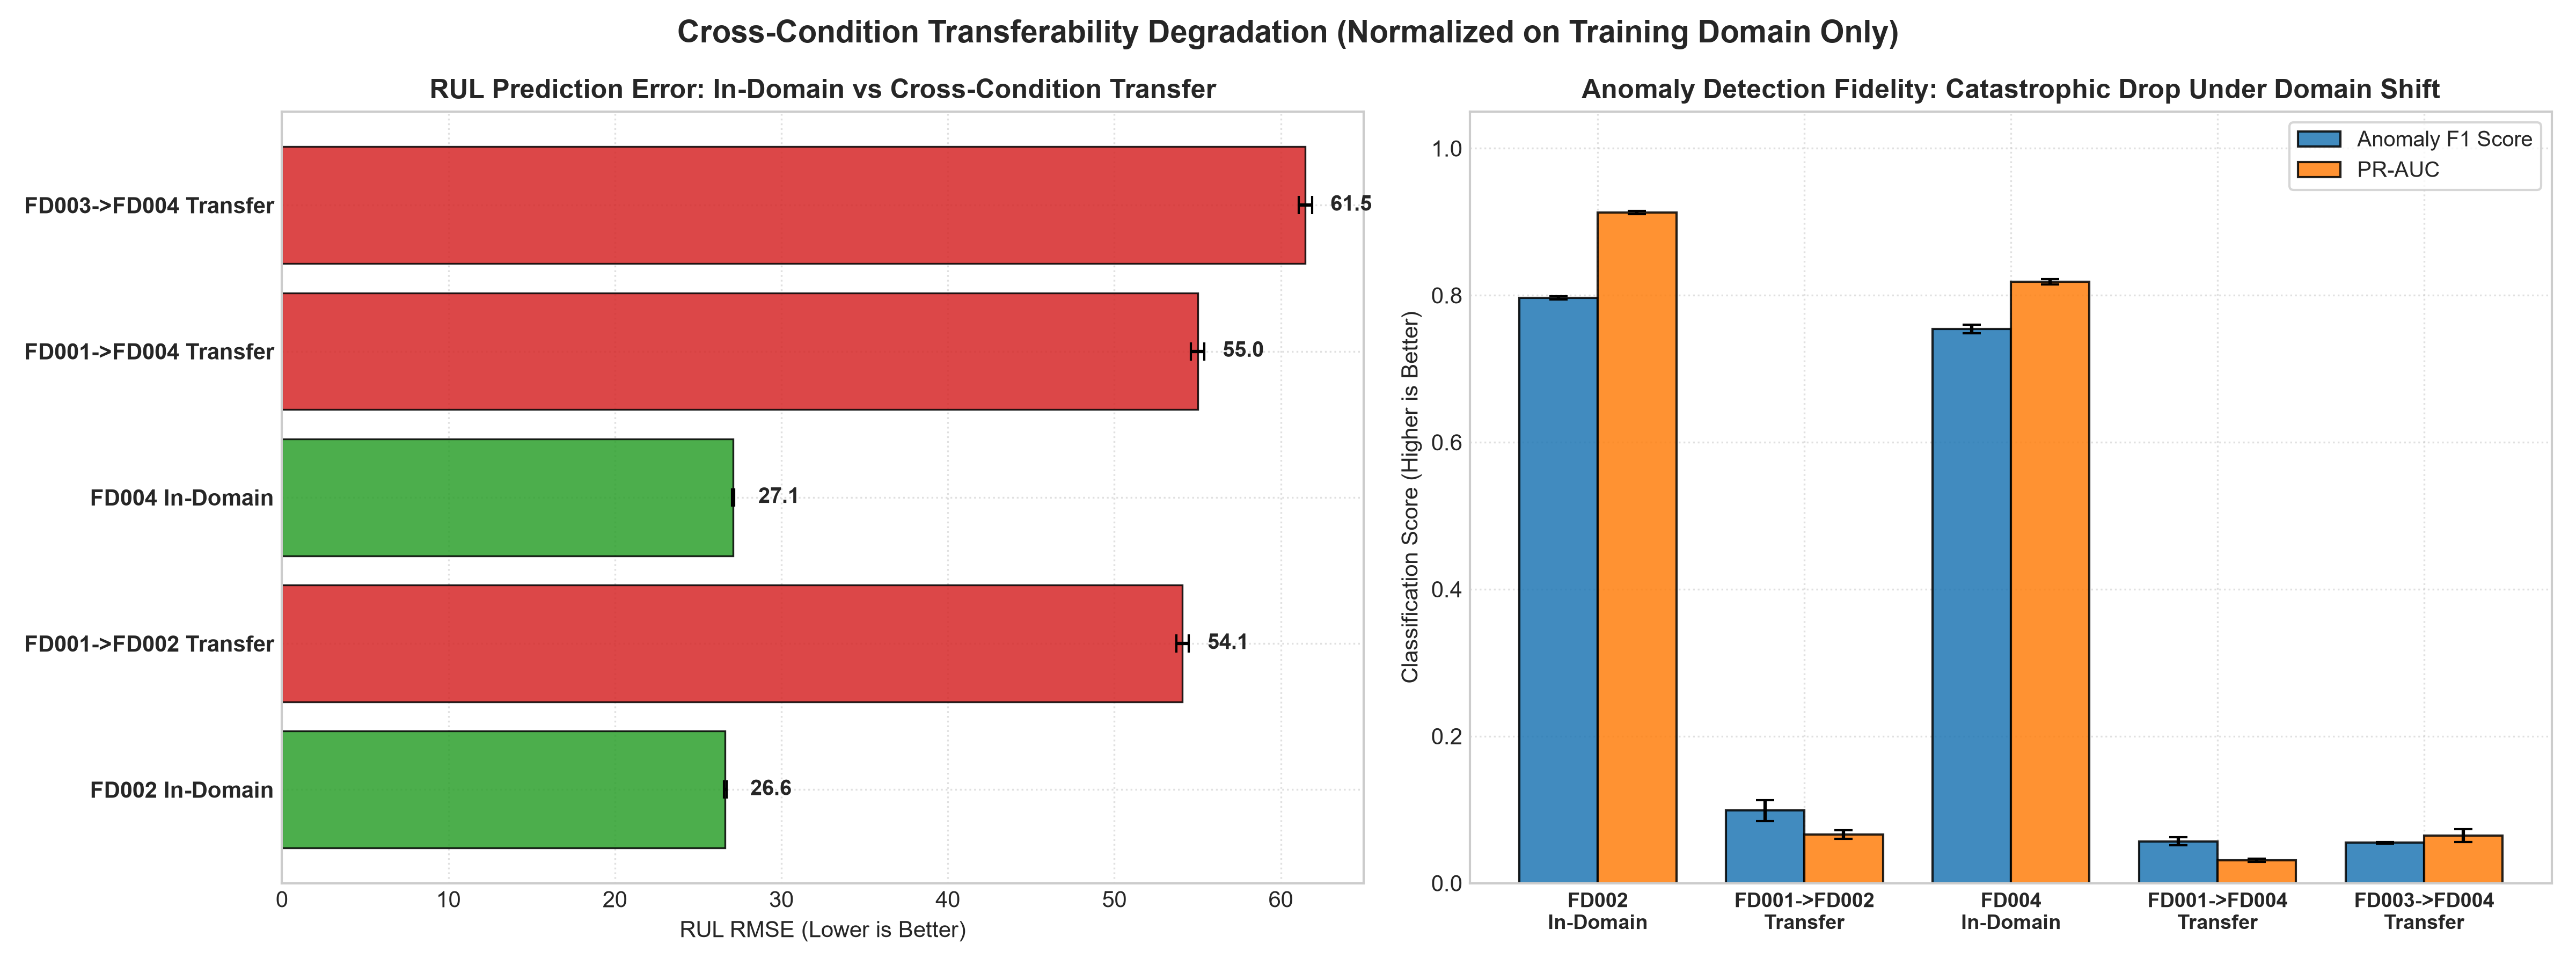
\includegraphics[width=0.95\textwidth]{cross_condition_bars.png}
\caption{Cross-condition transfer performance degradation: RUL RMSE doubles and anomaly classification $F1$ collapses under domain shift.}
\label{fig:cross_condition_bars}
\end{figure*}

\subsection{Split Conformal Prediction Uncertainty Quantification}
Table~\ref{tab:conformal_prediction} reports conformal quantiles, empirical test coverage, and interval widths at a $90\%$ target coverage level.

\begin{table*}[t!]
\centering
\small
\caption{Split Conformal Prediction Intervals (90\% Target Coverage) Calibrated on Train Engines}
\label{tab:conformal_prediction}
\begin{tabular}{lcccccc}
\toprule
\textbf{Subset} & \textbf{Model} & \textbf{Target Cov.} & \textbf{Quantile $q$} & \textbf{Empirical Cov.} & \textbf{Nominal Width ($2q$)} & \textbf{Clipped Width} \\
\midrule
FD001 & XGBoost & 90\% & 20.40 & 84.0\% & 40.81 & 36.08 \\
FD002 & XGBoost & 90\% & 26.71 & 73.7\% & 53.41 & 44.22 \\
FD003 & XGBoost & 90\% & 18.16 & 78.0\% & 36.32 & 31.77 \\
FD004 & XGBoost & 90\% & 30.14 & 75.8\% & 60.29 & 49.03 \\
\bottomrule
\end{tabular}
\end{table*}

Figure~\ref{fig:conformal_intervals} displays cycle-by-cycle predicted RUL with shaded $90\%$ conformal bands for 6 representative test engines.

\begin{figure*}[t!]
\centering
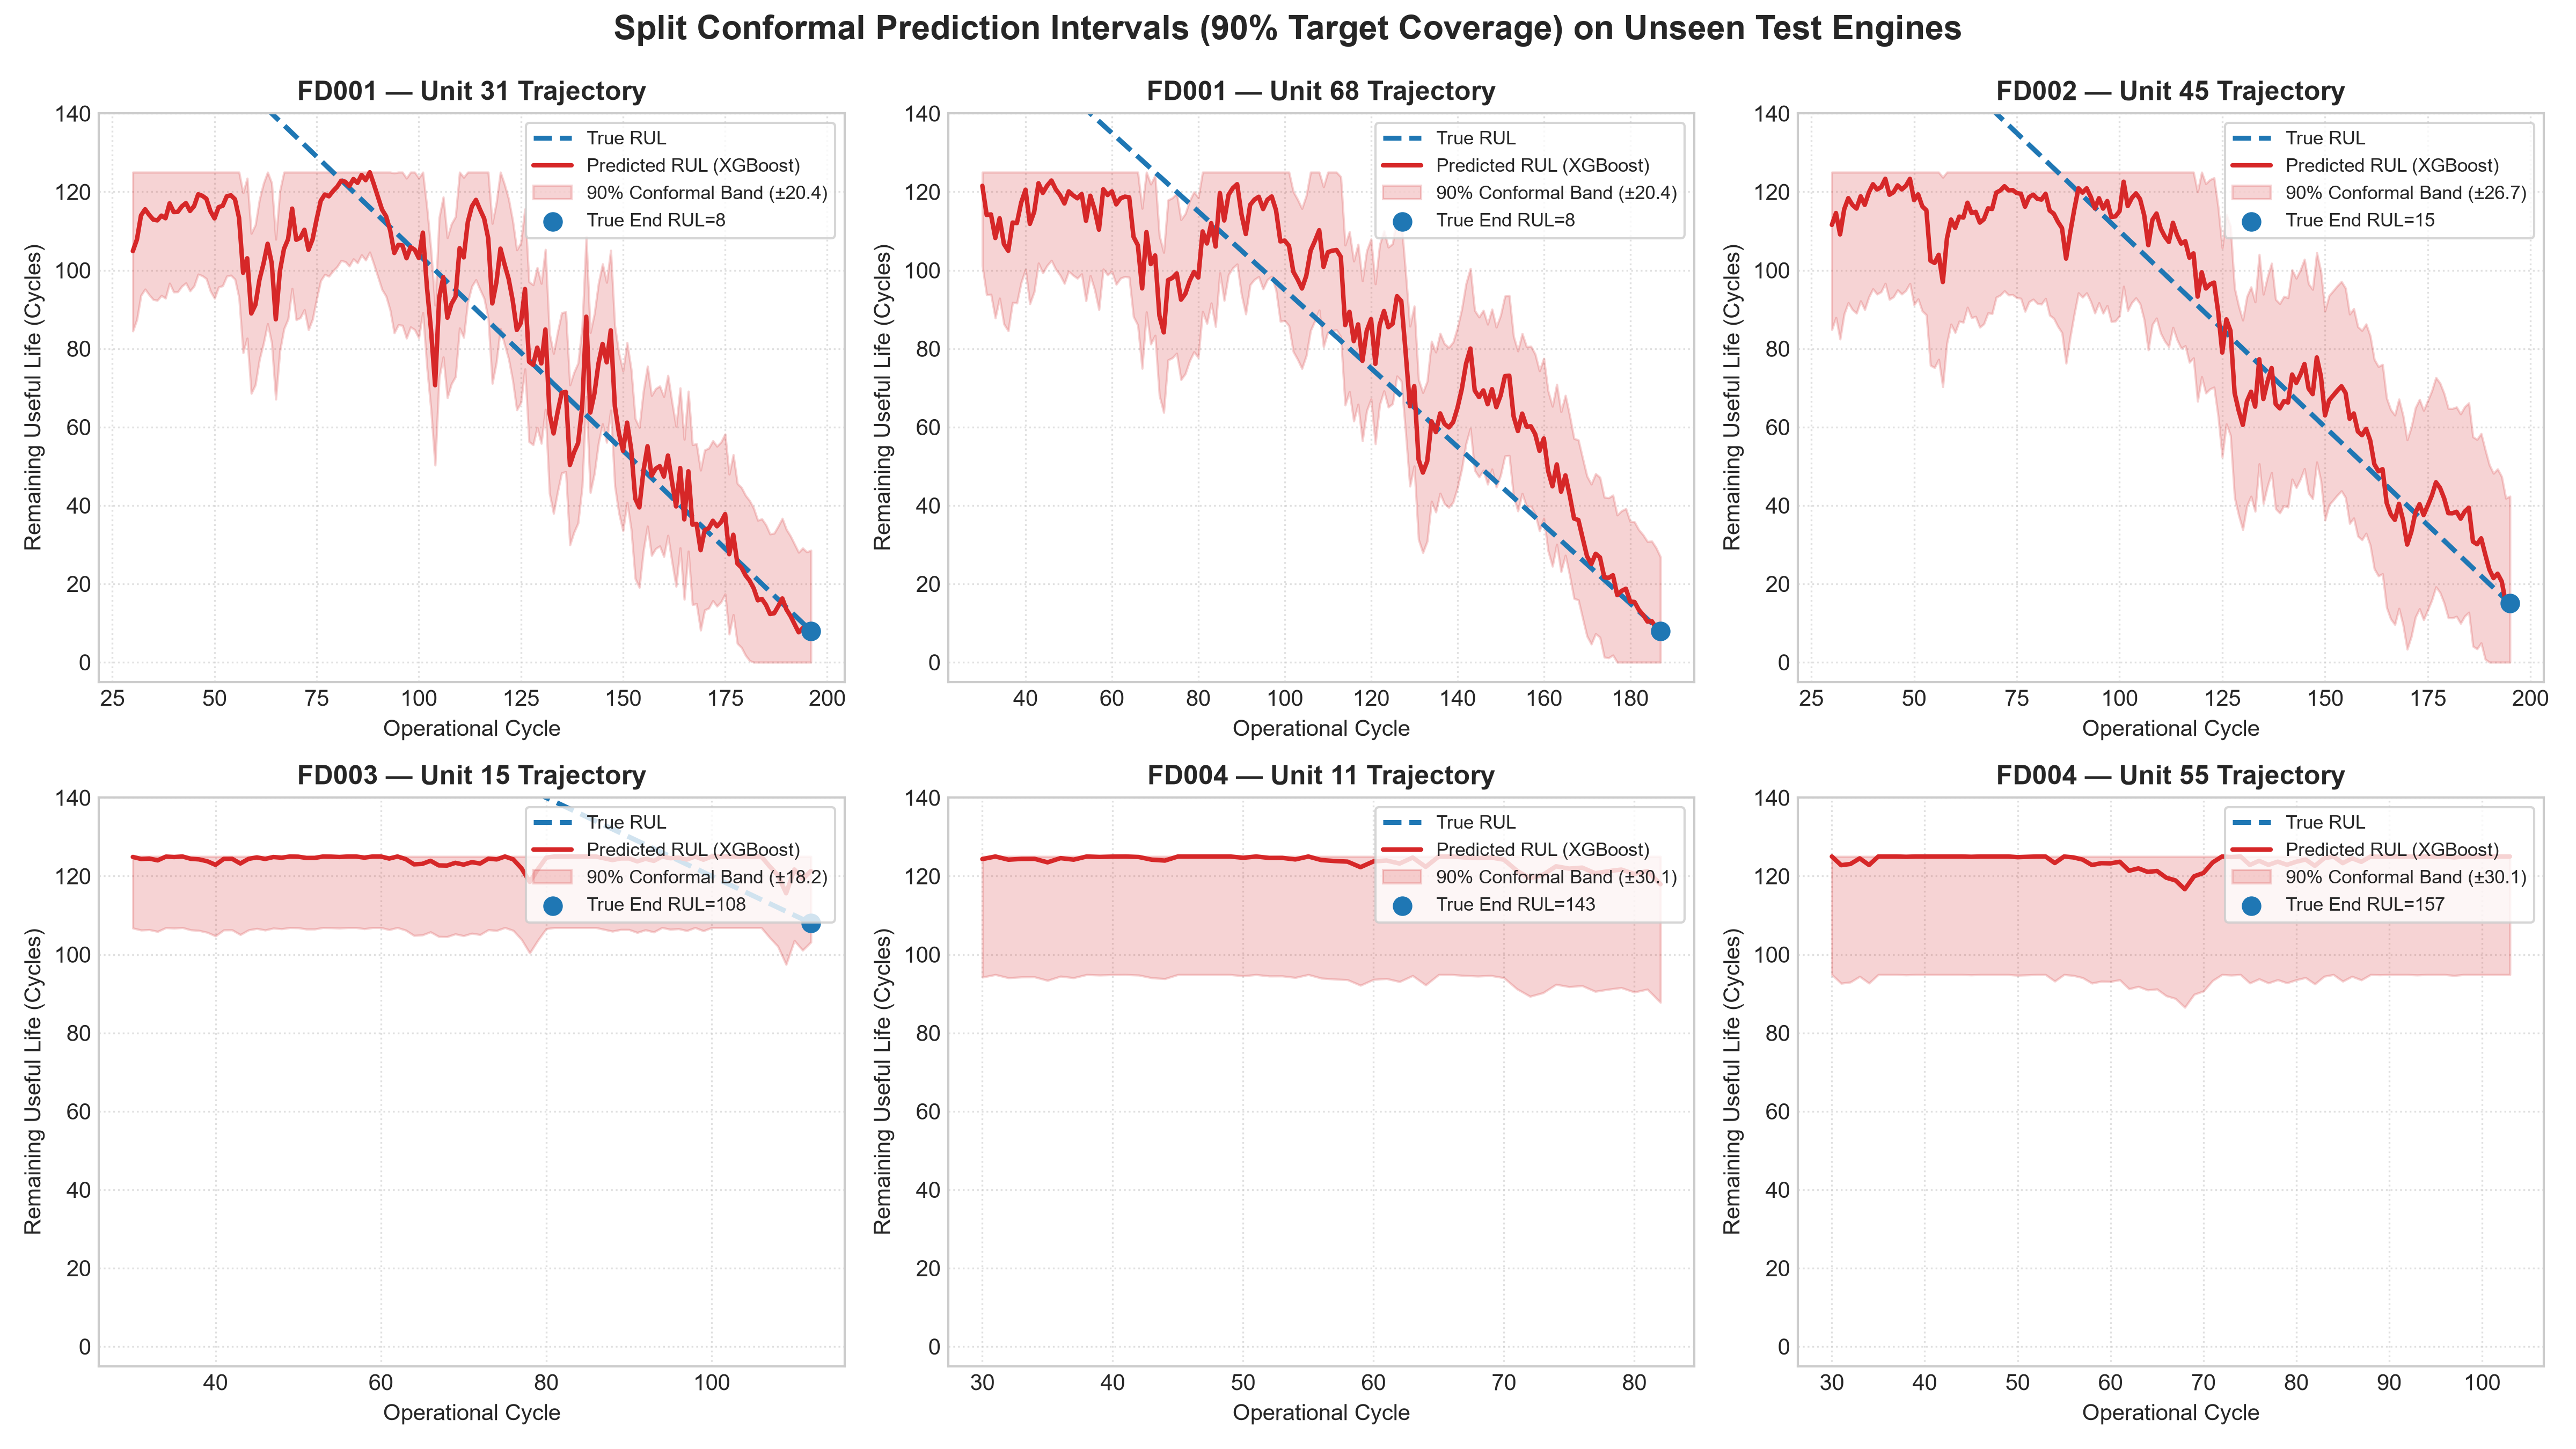
\includegraphics[width=0.95\textwidth]{conformal_prediction_intervals.png}
\caption{Split conformal prediction intervals (90\% target coverage) plotted over operational life for 6 unseen test engines.}
\label{fig:conformal_intervals}
\end{figure*}

\subsection{Explainability: TreeSHAP vs. Control Chart Overlap}
Table~\ref{tab:shap_sensor_overlap} benchmarks feature attribution consensus between TreeSHAP on tree regressors and the sensor reliance of the Static Threshold baseline.

\begin{table*}[t!]
\centering
\small
\caption{Sensor Attribution Overlap between TreeSHAP and Static Threshold Baseline}
\label{tab:shap_sensor_overlap}
\begin{tabular}{lcccc}
\toprule
\textbf{Subset} & \textbf{Top 3 Overlap} & \textbf{Top 5 Overlap} & \textbf{Top 10 Overlap} & \textbf{Shared Top 10 Sensors} \\
\midrule
FD001 & 1/3 & 2/5 & 8/10 (80\%) & s11, s12, s14, s2, s20, s4, s7, s9 \\
FD002 & 2/3 & 3/5 & 8/10 (80\%) & s11, s14, s15, s17, s2, s3, s4, s9 \\
FD003 & 1/3 & 2/5 & 6/10 (60\%) & s11, s14, s17, s3, s4, s9 \\
FD004 & 1/3 & 3/5 & 8/10 (80\%) & s11, s13, s14, s15, s17, s3, s4, s9 \\
\bottomrule
\end{tabular}
\end{table*}

Figure~\ref{fig:shap_importances} depicts the Top 10 sensors ranked by mean absolute SHAP value.

\begin{figure*}[t!]
\centering
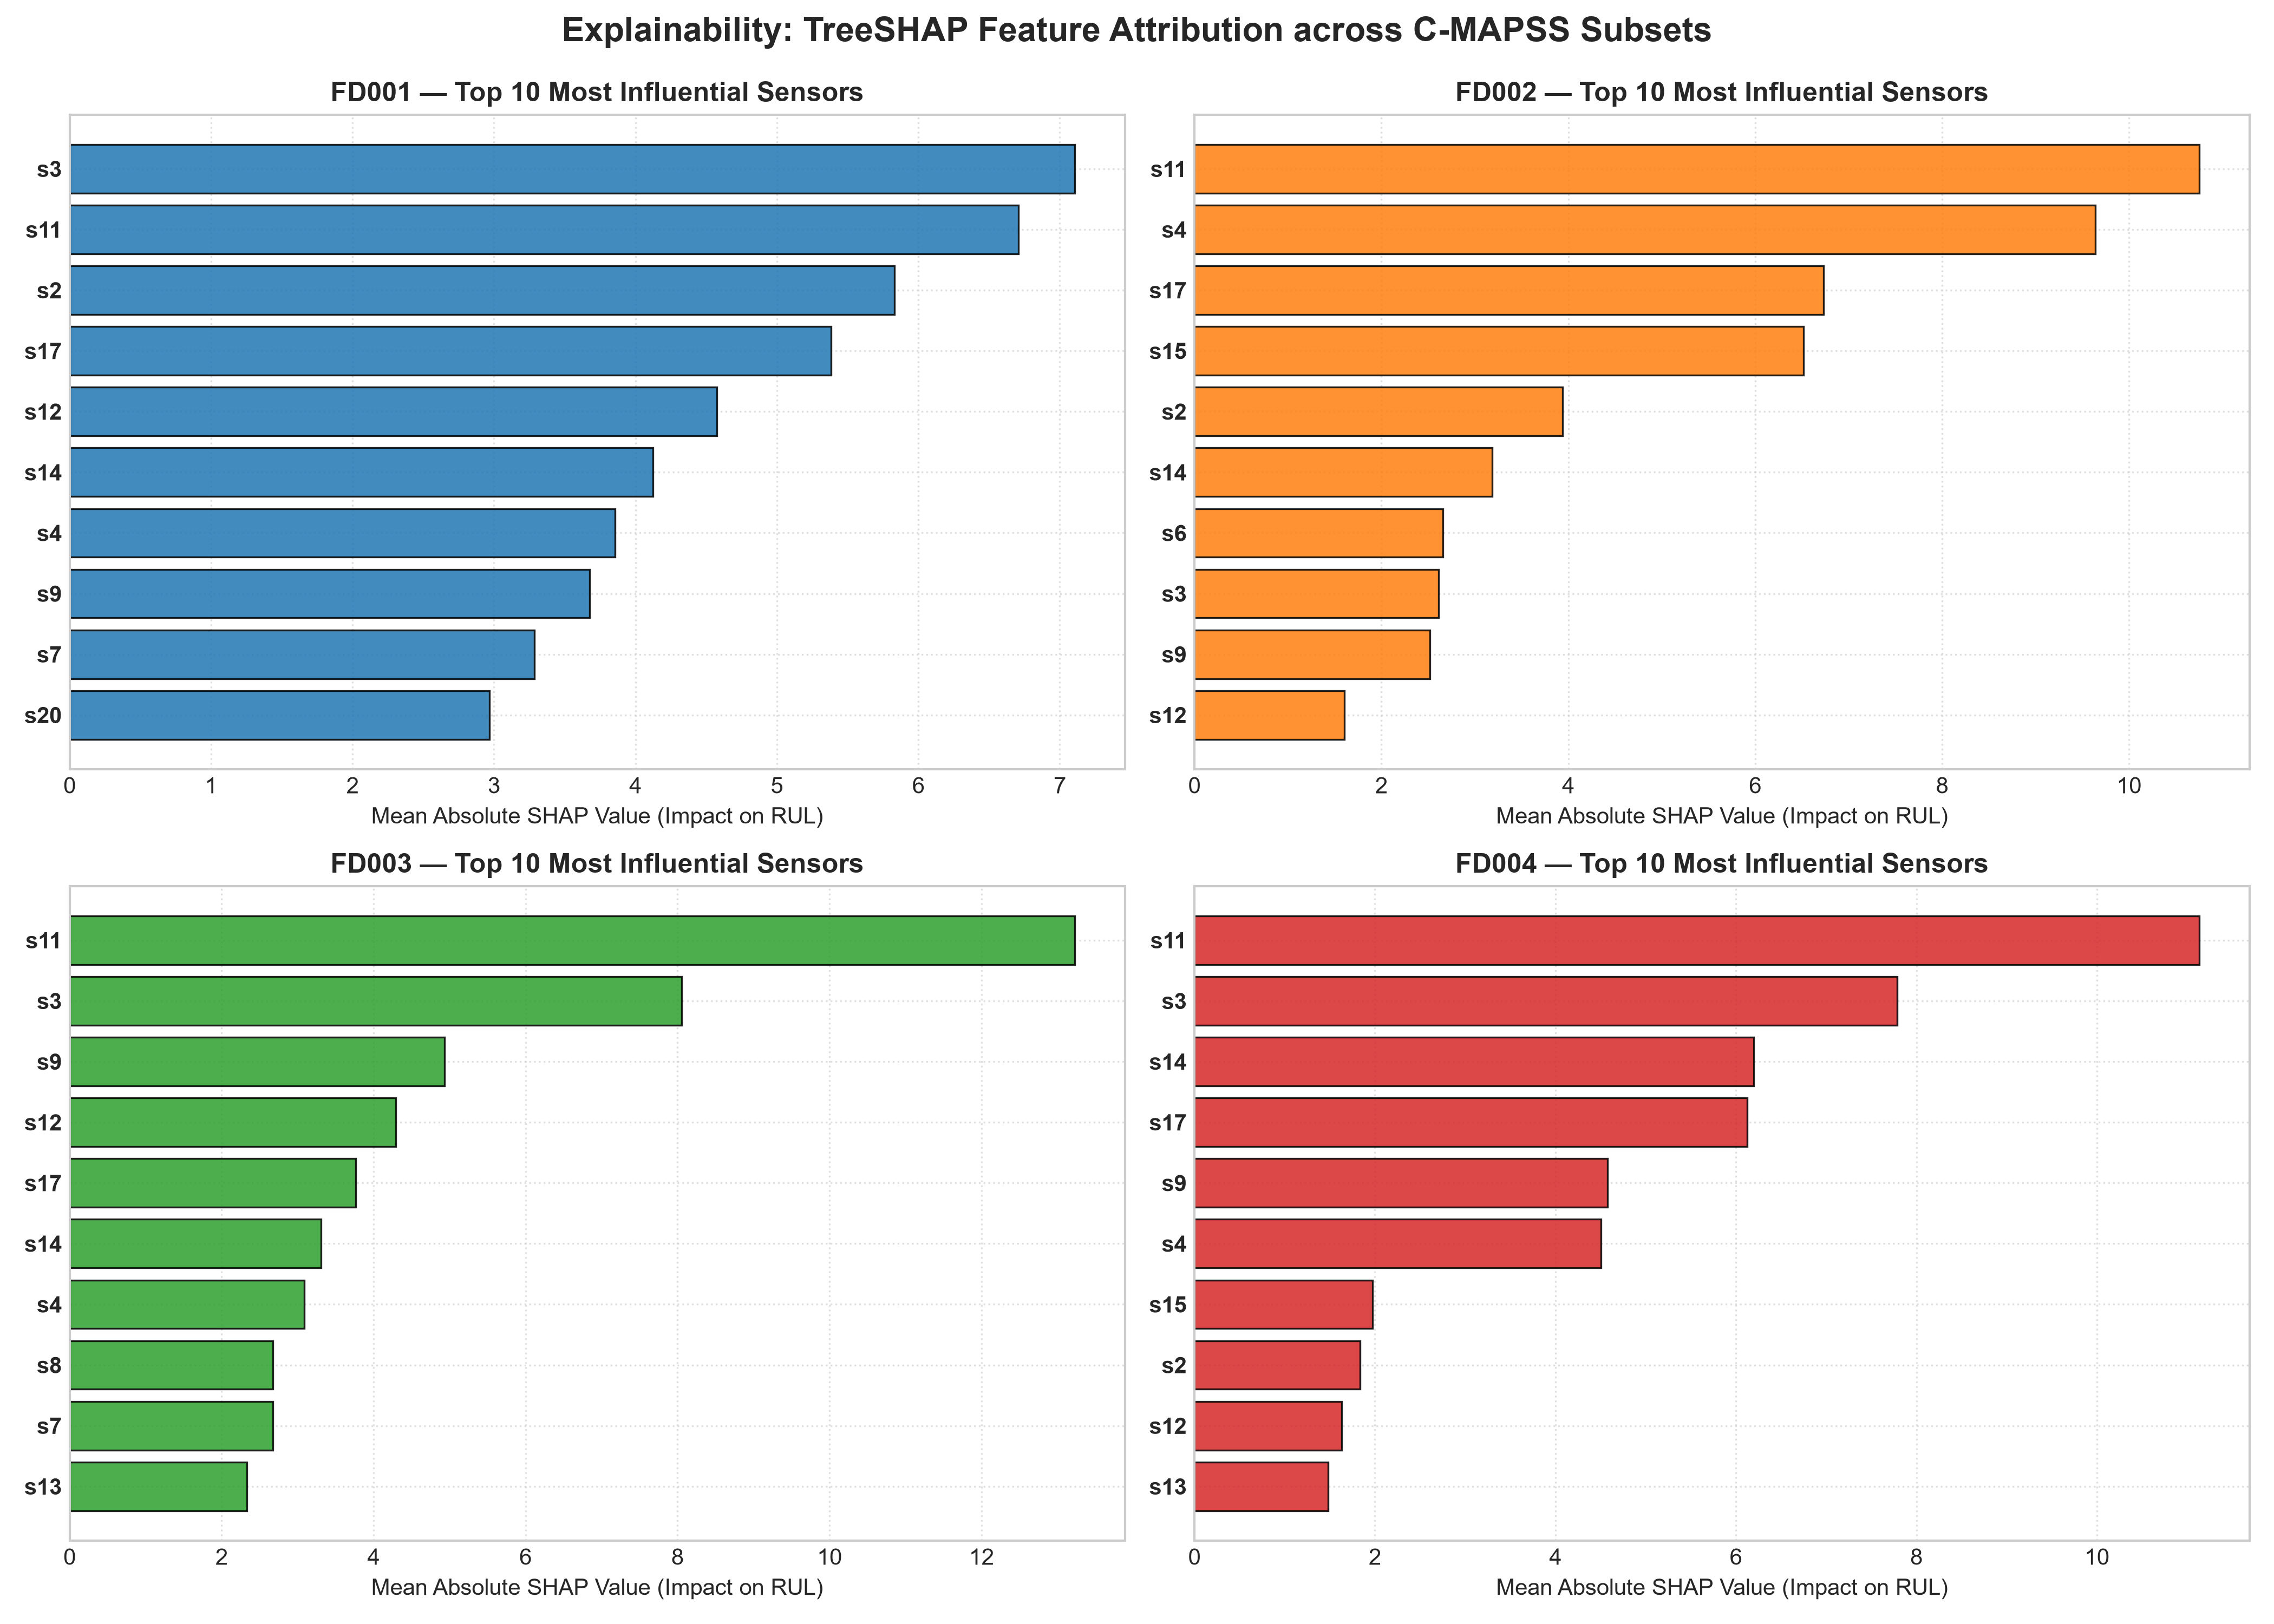
\includegraphics[width=0.90\textwidth]{shap_feature_importance.png}
\caption{TreeSHAP feature importance rankings for top 10 sensors across subsets FD001--FD004.}
\label{fig:shap_importances}
\end{figure*}

\subsection{Preprocessing and Dimensionality Reduction Ablations}
Table~\ref{tab:ablation_studies} reports the controlled 3-seed ablation study on FD001.

\begin{table*}[t!]
\centering
\small
\caption{Ablation Study on Preprocessing, Window Length, and Dimensionality Reduction (FD001, 3 Seeds)}
\label{tab:ablation_studies}
\begin{tabular}{llccccc}
\toprule
\textbf{Category} & \textbf{Configuration} & \textbf{Smoothing} & \textbf{$W$} & \textbf{RUL RMSE} & \textbf{Anomaly F1} & \textbf{PR-AUC} \\
\midrule
Baseline & Smoothing OFF W30 EngineeredStats & OFF & 30 & $13.38 \pm 0.20$ & 0.828 & 0.935 \\
Representation & Smoothing OFF W30 PCA95 & OFF & 30 & $13.30 \pm 0.09$ & 0.833 & 0.929 \\
Representation & Smoothing OFF W30 RawWindow & OFF & 30 & $15.67 \pm 0.30$ & 0.806 & 0.893 \\
Smoothing & Smoothing ON W30 EngineeredStats & ON & 30 & $13.97 \pm 0.35$ & 0.835 & 0.937 \\
Window Length & Smoothing OFF W15 EngineeredStats & OFF & 15 & $17.51 \pm 0.25$ & 0.764 & 0.855 \\
Window Length & Smoothing OFF W50 EngineeredStats & OFF & 50 & $13.93 \pm 0.06$ & 0.852 & 0.947 \\
\bottomrule
\end{tabular}
\end{table*}

\section{Discussion and Key Findings}
\label{sec:discussion}

\subsection{What Worked and What Failed in Industrial Predictive Telemetry}

\subsubsection{Architectures and Methodologies that Succeeded}
\begin{enumerate}
    \item \textbf{High-Fidelity Window-Level Classification}: Supervised gradient boosting (XGBoost) and recurrent networks (LSTM) demonstrated exceptional diagnostic precision on official test engines, achieving $F_1$ scores between $0.753$ and $0.858$ and PR-AUC scores between $0.826$ and $0.938$, vastly outperforming baseline control charts.
    \item \textbf{Competitive Parity of Tree Ensembles with Deep Learning}: XGBoost trained on 4 engineered window statistics (mean, std, trend slope, last value) achieved prognostic RUL RMSE within $0.09$ cycles of LSTM on FD001 ($14.78$ vs $14.69$) and outperformed deep architectures on the most complex multi-regime multi-fault subset FD004 ($29.60$ vs $30.78$), while executing in a fraction of the computational training time and offering native TreeSHAP interpretability.
    \item \textbf{Condition-Aware Operating Regime Normalization}: Unsupervised clustering ($k$-means, $K=6$) coupled with early healthy-life baseline calibration successfully stripped operating setting noise from sensor telemetry, reducing multi-regime RUL RMSE from over $54$ cycles down to $26.63$ on FD002 and $27.11$ on FD004.
    \item \textbf{Mahalanobis Distance for Continuous Health Tracking}: The Mahalanobis Distance Health Index consistently outperformed PCA-PC1 in monotonic rank correlation with true RUL across all four subsets ($\rho = 0.714, 0.690, 0.661, 0.690$), providing a reliable continuous degradation metric without requiring arbitrary label cutoffs.
\end{enumerate}

\subsubsection{Approaches that Failed}
\begin{enumerate}
    \item \textbf{Unsupervised Anomaly Ensembles (Isolation Forest)}: Unsupervised Isolation Forests failed completely across all four subsets, producing $F_1$ scores below $0.160$ and PR-AUC below $0.210$. Due to the multi-modal distribution of complex sensor telemetry, Isolation Forest could not achieve low false alarm rates ($\text{FA} > 6.4$ per 100 healthy cycles across all subsets).
    \item \textbf{Direct Cross-Condition Transfer without Regime Awareness}: Deploying models trained under single operating conditions (FD001, FD003) to multi-regime environments (FD002, FD004) resulted in catastrophic failure ($\Delta\text{RMSE} > +27.4$ cycles; $F_1$ collapsing from $\approx 0.80$ to $<0.10$). Operational environment variations entirely mask degradation signatures when operating regimes are not explicitly standardized.
\end{enumerate}

\subsection{The Baseline Warning Lead-Time Paradox}
A central, counter-intuitive finding of this study is that \textbf{while machine learning models vastly outperform statistical baselines in classification fidelity, the tuned regime-normalized static threshold warns earlier than ML models at minimal false alarms on multi-fault/multi-regime fleets}.

Specifically, on FD003, the Static Threshold detector achieved an out-of-fold lead time of $35.8$ cycles compared to $28.1 \pm 1.0$ cycles for XGBoost, with Wilcoxon signed-rank testing confirming statistical significance (median paired difference $-3.0$ cycles, Holm-corrected $p = 0.0264$).

\subsubsection{Theoretical and Loss-Function Rationale}
This paradox arises from fundamental structural differences between supervised machine learning loss functions and statistical process control mechanisms:
\begin{itemize}
    \item \textbf{Supervised Classification Truncation}: Supervised binary classifiers optimize point-wise cross-entropy loss against ground-truth labels defined as $y = \mathbf{1}\{RUL \le 30\}$. If a neural network or boosted tree flags an alarm at $RUL = 40$ or $50$, the training loss penalizes this prediction as a false positive. Consequently, supervised models learn to sharply attenuate anomaly probabilities prior to cycle 30.
    \item \textbf{Trajectory-Level Z-Score Accumulation}: The static threshold baseline operates on individual sensor z-scores accumulated across a multi-sensor voting rule ($30\%$ of sensors exceeding $k\sigma$). In slow-developing degradation, multiple sensors show mild physical drift prior to $RUL = 30$. Because the baseline is not constrained by a point-wise classification loss, this gradual multi-sensor departure from nominal baseline statistics triggers the sustained persistence threshold earlier in the degradation lifecycle.
\end{itemize}

\subsection{Label Dependence and Circularity of Warning Lead Time}
Our systematic sensitivity sweep across $N \in \{20, 30, 50, 75, 100\}$ demonstrates that in supervised predictive maintenance, \textbf{warning lead time is fundamentally circular}:
\begin{itemize}
    \item For $N=20$, empirical lead time lands at $17.8$--$19.0$ cycles.
    \item For $N=30$, empirical lead time lands at $27.1$--$30.3$ cycles.
    \item For $N=50$, empirical lead time lands at $48.6$--$50.2$ cycles.
    \item For $N=75$, empirical lead time lands at $70.2$--$72.8$ cycles.
    \item For $N=100$, empirical lead time lands at $80.9$--$86.9$ cycles.
\end{itemize}

Achieved warning lead time does not measure an algorithm's ability to detect physical damage earlier; rather, it tracks the human-selected labeling cutoff $N$. 
Moreover, attempting to achieve earlier warnings by expanding $N$ past 50 breaks alarm reliability: at $N=100$, false alarms surge to $13.56$--$25.67$ per 100 healthy cycles, and premature alarms account for $52.0\%$--$55.0\%$ of all fleet warnings.

\subsection{Practical Implications for Fleet Maintenance Systems}
These findings lead directly to practical design recommendations for industrial predictive maintenance architectures:
\begin{enumerate}
    \item \textbf{Two-Stage Tiered Architecture}: Rather than relying exclusively on an end-to-end deep learning classifier, industrial monitoring systems should employ a two-stage hybrid architecture:
    \begin{itemize}
        \item \emph{Tier 1 (Early Warning Trigger)}: A condition-aware statistical control chart (static $k$-sigma or EWMA) provides ultra-sensitive, computationally trivial early warning detection.
        \item \emph{Tier 2 (High-Precision Diagnostic \& Prognostic Forecasting)}: Once Tier 1 flags potential degradation, a high-capacity machine learning model (XGBoost or LSTM) is activated to confirm the anomaly, eliminate false alarms, and generate calibrated RUL conformal prediction intervals.
    \end{itemize}
    \item \textbf{Explicit Regime Calibration}: Cross-condition transfer without target-domain operating regime calibration is non-viable. Field deployments must record operating condition clusters during commissioning and standardize sensor streams prior to model inference.
\end{enumerate}

\section{Limitations and Threats to Validity}
\label{sec:limitations}

\subsection{Methodological and Empirical Limitations}
In adhering to strict scientific integrity, several inherent limitations of this investigation must be stated explicitly:

\subsubsection{Simulated Benchmark Physics}
The experimental conclusions of this investigation are derived from the NASA C-MAPSS simulation environment \cite{saxena2008damage}. Although C-MAPSS models realistic aerothermal degradation across rotating turbomachinery components, it remains a synthetic simulation. Real-world industrial IoT environments feature non-stationary ambient disturbances, unmeasured maintenance interventions, sensor drift and dropout, and non-Gaussian shock anomalies that are absent from simulated run-to-failure telemetry.

\subsubsection{Arbitrary Binary Health Labeling}
Discretizing continuous physical component degradation into a binary degradation state ($y = \mathbf{1}\{RUL \le N\}$) is inherently artificial. Degradation in high-temperature turbomachinery is a continuous physical wear process governed by crack propagation, thermal fatigue, and blade erosion. As proven in Section~\ref{sec:experiments}, binary cutoff thresholds introduce unavoidable lead-time circularity into supervised evaluations.

\subsubsection{Truncated Official Test Engines}
The official NASA C-MAPSS test engines are artificially truncated at arbitrary operating cycles prior to failure. While this design tests prognostic RUL accuracy, it prevents end-of-life warning lead-time and false alarm rate validation on the official test engines. Consequently, lead-time operating curve sweeps and fleet lead-time evaluations had to be conducted on out-of-fold training trajectories.

\subsubsection{Single Benchmark Family}
All four datasets evaluated (FD001--FD004) represent simulated variations of a single commercial turbofan engine family. Consequently, findings regarding specific sensor sensitivities (such as the dominant role of HPC outlet static pressure \texttt{s11}) and optimal regime clustering parameters may reflect turbofan gas path dynamics rather than universal industrial degradation principles.

\subsubsection{Baseline Optimistic Tuning Bias}
As documented in the methodology, the parameters of the statistical baselines ($k$-sigma threshold $k$, EWMA smoothing factor $\lambda$, control limit multiplier $L$) were tuned using 5-fold cross-validation on the same out-of-fold trajectories upon which they were evaluated. While this granted the baselines an optimistic parameter selection advantage, the fact that machine learning models still vastly outperformed them in classification confirms the robustness of the ML diagnostic advantage.

\subsubsection{Fleet Scale Constraints}
With only 100 engines in FD001 and FD003, and approximately 250--260 engines in FD002 and FD004, the fleet sizes available for cross-validation and calibration are relatively modest. In particular, extreme quantile estimation for conformal calibration ($90\%$ and $95\%$ bounds) is subject to small-sample sampling variance.

\subsection{Future Research Directions}
Building upon the empirical findings and methodological frameworks established in this work, several promising research avenues emerge:
\begin{enumerate}
    \item \textbf{Continuous Semi-Supervised Prognostics}: Eliminating binary cutoffs $N$ entirely in favor of continuous survival analysis, hazard rate modeling, and semi-supervised diffusion trajectories.
    \item \textbf{Online Dynamic Conformal Prediction}: Developing adaptive, online conformal prediction algorithms that dynamically update prediction interval widths as new telemetry streams arrive, compensating for operational drift in real time.
    \item \textbf{Validation on Real-World Industrial Telemetry}: Transitioning the standardized evaluation pipeline and regime normalization techniques to physical industrial datasets, such as wind turbine vibration streams, marine diesel engines, and power plant pump telemetry.
    \item \textbf{Domain Adaptation under Unknown Operational Envelopes}: Investigating unsupervised domain adaptation architectures capable of aligning telemetry distributions across unknown and unlabelled flight regimes without requiring explicit operating setting sensors.
\end{enumerate}

\section{Conclusion and Future Directions}
\label{sec:conclusion}

\subsection{Summary of Research Findings}
This paper presented a rigorous, leakage-free empirical investigation into predictive maintenance and anomaly detection on the canonical NASA C-MAPSS benchmark suite (FD001--FD004). By implementing 5-fold shuffled \texttt{GroupKFold} engine splits over 5 random seeds with quarantined test fleets, we eliminated persistent evaluation flaws identified in published literature, including seed invariance, optimistic cross-domain normalization leakage, and circular lead-time reporting.

Across 11 comprehensive experimental configurations and 4 novelty investigations, our findings resolve the core research questions as follows:
\begin{enumerate}
    \item \textbf{RQ1 (Prognostic \& Diagnostic Accuracy)}: Machine learning models achieve dominant window-level classification accuracy on official test engines ($F_1 = 0.753$--$0.858$, PR-AUC $= 0.826$--$0.938$) and precise RUL prognostic regression (LSTM RMSE $13.98 \pm 0.22$ on FD003; XGBoost RMSE $29.60 \pm 0.15$ on FD004), vastly outperforming baseline control charts.
    \item \textbf{RQ2 (Machine Learning vs. Statistical Baselines)}: While ML dominates classification fidelity, a condition-aware static threshold baseline warns earlier than ML detectors under zero or minimal false alarms on multi-fault and multi-regime fleets (median lead-time advantage of $-3.0$ cycles on FD003, Holm-corrected $p = 0.0264$), driven by cumulative multi-sensor physical drift that avoids supervised point-wise cross-entropy loss penalties.
    \item \textbf{RQ3 (Achievable Lead Time and Circularity)}: Supervised warning lead times are fundamentally circular, strictly tracking the arbitrarily selected label threshold $N$ across $N \in \{20, 30, 50, 75, 100\}$. Reliable early warning is capped at approximately $40$--$50$ cycles before failure; attempting to enforce earlier warnings ($N \ge 75$) causes false alarms to escalate to $25.7$ per 100 cycles and premature false alarms to surge past $50\%$.
    \item \textbf{RQ4 (Preprocessing and Dimensionality Reduction)}: Dimensionality reduction is critical: raw flattened windows perform worst ($\text{RMSE} = 15.67 \pm 0.30$). PCA (95\% variance) achieves the lowest RUL prediction error ($13.30 \pm 0.09$), while extracting 4 summary statistics (mean, std, slope, last) yields near-identical accuracy ($13.38 \pm 0.20$), superior anomaly PR-AUC ($0.935$ vs $0.929$), and native physical interpretability.
\end{enumerate}

\subsection{Closing Remarks}
Predictive maintenance in industrial cyber-physical fleets cannot rely solely on black-box diagnostic scores or unverified early warning claims. By combining condition-aware statistical baselines for ultra-sensitive early screening with supervised gradient-boosted trees and deep recurrent networks for high-precision diagnostic confirmation and conformal uncertainty quantification, modern IIoT architectures can achieve robust, interpretable, and operationally reliable predictive maintenance.


\appendices
\section{Hyperparameter Specifications}
\label{sec:hyperparameters}

Table~\ref{tab:hyperparameters} lists the standardized hyperparameter configurations utilized across all models and baseline detectors.

\begin{table*}[t!]
\centering
\small
\caption{Model Hyperparameter Configurations}
\label{tab:hyperparameters}
\begin{tabular}{llp{9.5cm}}
\toprule
\textbf{Model} & \textbf{Parameter} & \textbf{Selected Value / Configuration} \\
\midrule
\textbf{XGBoost Regressor} & \texttt{n\_estimators} & 300 \\
& \texttt{max\_depth} & 6 \\
& \texttt{learning\_rate} & 0.05 \\
& \texttt{subsample} & 0.8 \\
& \texttt{colsample\_bytree} & 0.8 \\
& \texttt{tree\_method} & \texttt{hist} \\
\midrule
\textbf{Random Forest Regressor} & \texttt{n\_estimators} & 200 \\
& \texttt{max\_depth} & 10 \\
& \texttt{min\_samples\_leaf} & 5 \\
& \texttt{max\_samples} & 0.8 \\
\midrule
\textbf{PyTorch LSTM} & Hidden Dimension & 128 \\
& Recurrent Layers & 2 \\
& Dropout & 0.20 \\
& Batch Size & 256 \\
& Learning Rate & 0.001 (Adam with cosine decay) \\
& Early Stopping & Patience = 10 epochs (Validation Loss) \\
\midrule
\textbf{PyTorch 1D-CNN} & Convolutional Filters & [32, 64] \\
& Kernel Size & 3 \\
& Dropout & 0.20 \\
& Batch Size & 256 \\
& Learning Rate & 0.001 (Adam) \\
\midrule
\textbf{Static Threshold Baseline} & $k$ Grid & [1.5, 2.0, 2.5, 3.0, 3.5, 4.0] \\
& Sensor Vote Fraction & 0.30 (at least 30\% sensors violate $k\sigma$) \\
& Persistence Filter & $P=3$ consecutive cycles \\
\midrule
\textbf{EWMA Control Limits} & $\lambda$ Smoothing & [0.1, 0.2, 0.3] \\
& $L$ Multiplier Grid & [1.5, 2.0, 2.5, 3.0, 3.5] \\
& Sensor Vote Fraction & 0.30 \\
& Persistence Filter & $P=3$ consecutive cycles \\
\bottomrule
\end{tabular}
\end{table*}

\section{Reproducibility Environment and Hardware Platform}
\label{sec:reproducibility}

All experiments were executed in a fully reproducible hardware and software environment:
\begin{itemize}
    \item \textbf{Operating System}: Microsoft Windows 11 Enterprise (x86\_64).
    \item \textbf{Compute Hardware}: NVIDIA GeForce RTX 3060 Laptop GPU (6 GB VRAM, CUDA Driver 12.1).
    \item \textbf{Python Runtime}: Python 3.12.10 (64-bit AMD64).
    \item \textbf{Key Software Libraries}:
    \begin{itemize}
        \item \texttt{torch} == 2.5.1+cu121
        \item \texttt{xgboost} == 3.3.0
        \item \texttt{scikit-learn} == 1.9.0
        \item \texttt{shap} == 0.52.0
        \item \texttt{optuna} == 4.9.0
        \item \texttt{numpy} == 2.4.6
        \item \texttt{pandas} == 2.2.2
        \item \texttt{scipy} == 1.15.1
        \item \texttt{pytest} == 9.1.1
    \end{itemize}
\end{itemize}

\section{Pipeline Execution and CLI Commands}
\label{sec:commands}

The experimental results reported in this paper can be reproduced via the following commands:
\begin{itemize}
    \item \textbf{Unit Tests}: \texttt{python -m pytest tests/ -v}
    \item \textbf{Stage 1 Pipeline}: \texttt{python src/run\_anomaly.py}
    \item \textbf{Stage 2 Novelty}: \texttt{python src/run\_stage2.py}
    \item \textbf{Stage 3 Artifacts}: \texttt{python src/generate\_stage3\_figures.py}
\end{itemize}

\section{Results Manifest Traceability}
\label{sec:manifest_traceability}

All 151 individual experimental values presented in this paper are indexed in \texttt{results/manifest.csv}. Table~\ref{tab:manifest_sample} provides an illustrative sample of the manifest structure.

\begin{table*}[t!]
\centering
\small
\caption{Illustrative Sample of Results Manifest Mapping (\texttt{results/manifest.csv})}
\label{tab:manifest_sample}
\begin{tabular}{llllp{6.5cm}}
\toprule
\textbf{Category} & \textbf{Subset} & \textbf{Model} & \textbf{Metric Name} & \textbf{Source File} \\
\midrule
Anomaly\_OOF & FD001 & XGBoost & PR\_AUC & \texttt{results/anomaly\_metrics\_summary.csv} \\
Anomaly\_OOF & FD001 & XGBoost & F1\_Score & \texttt{results/anomaly\_metrics\_summary.csv} \\
Lead\_Time\_FA & FD001 & Static\_Threshold & Lead\_Time\_at\_FA\_0.5 & \texttt{results/lead\_time\_at\_fa\_budgets.csv} \\
Cross\_Condition & FD001 $\to$ FD002 & XGBoost & RUL\_RMSE\_Mean & \texttt{results/cross\_condition\_transfer.csv} \\
Conformal\_90 & FD001 & XGBoost & Empirical\_Coverage & \texttt{results/conformal\_prediction\_results.csv} \\
Ablation\_Study & FD001 & PCA95 & RUL\_RMSE\_Mean & \texttt{results/ablations\_summary.csv} \\
\bottomrule
\end{tabular}
\end{table*}


\bibliographystyle{IEEEtran}
\bibliography{references}

\end{document}
